\documentclass[b4paper, 10pt]{ctexart}
\usepackage[margin=0.5cm]{geometry}
\usepackage{multicol}

\usepackage{amsmath,amssymb,amsthm}
\usepackage{mathrsfs}
\usepackage{thmtools}
\usepackage{stmaryrd}

\usepackage{booktabs}
\usepackage[shortlabels]{enumitem}

\usepackage[colorlinks]{hyperref}
\usepackage{fontawesome5}

\usepackage{tikz-cd}

\usepackage{xargs}

% ctex 排版设置
\ctexset{
section = {
    beforeskip = {-1ex},
    afterskip = {-1ex},
},
subsection = {
    beforeskip = {-1ex},
    afterskip = {-1ex},
},
subsubsection = {
    beforeskip = {-1ex},
    afterskip = {-1ex},
},
}
\setlength{\parindent}{0pt} % 抑制首行缩进以减少空白
\setlist{nosep} % 抑制列表项之间的空白

% 数学符号
\newcommand*{\bb}[1]{\mathbb{#1}}
\newcommand*{\setN}{\mathbb{N}}
\newcommand*{\setZ}{\mathbb{Z}}
\newcommand*{\setQ}{\mathbb{Q}}
\newcommand*{\setR}{\mathbb{R}}
\newcommand*{\setC}{\mathbb{C}}
\newcommand*{\st}{\text{ s.t. }}
\newcommand*{\stab}{\text{stab}}
\newcommand*{\powerset}[1]{\mathscr{P}(#1)}
\newcommand*{\impl}{\Rightarrow}
\renewcommand*{\iff}{\Leftrightarrow}
\renewcommand*{\leq}{\leqslant}
\renewcommand*{\geq}{\geqslant}
\newcommand*{\nmsubgroupeq}{\trianglelefteqslant}
\newcommand*{\nmsubgroup}{\triangleleft}
\newcommand*{\gengroup}[1]{\langle #1 \rangle}
\newcommand*{\genring}[1]{[#1]}
\newcommand*{\genideal}[1]{(#1)}
\newcommand*{\genfield}[1]{\langle #1 \rangle}
\newcommand*{\ch}[1]{\text{ch}(#1)}
\newcommand*{\set}[1]{\{#1\}}
\newcommandx*\homo[3][3=]{#1 \overset{#3}{\rightarrow} #2}
\newcommandx*\mono[3][3=]{#1 \overset{#3}{\hookrightarrow} #2}
\newcommandx*\epi[3][3=]{#1 \overset{#3}{\twoheadrightarrow} #2}
\newcommandx*\iso[3][3=]{#1 \overunderset{\sim}{#3}{\rightarrow} #2}
\newcommand*{\ff}[1]{\bb{F}_{#1}}

% 数学环境
\declaretheoremstyle[
spaceabove=0pt, spacebelow=0pt,
headindent=-4pt,
notefont=\bfseries,notebraces={}{}
]{tight-thm}
\declaretheorem[name=, numbered=no, style=tight-thm]{theorem}

% 插入图片、表格的bug
\newenvironment{figurehere}
{\def\@captype{figure}}
{}
\newenvironment{tabhere}
{\def\@captype{table}}
{}

\usepackage{listings}

\begin{document}

\begin{multicols}{3}
\begin{center}
    {\Large 人工智能-马少平}

    Wheater

    \vspace*{-0.5em}

    \href{111}{\faGithub}

    \vspace*{-1em}
\end{center}

\section*{绪论}

\textbf{人工智能\ }  = “定义”+“算法”

“定义”:描述问题;“算法”:智能问题→计算问题

\textbf{深度学习存在的问题\ } 大数据/小样本、黑箱/可解释性、一次性学习/增量学习、固执己见/知错能改、猜测/理解

\textbf{人工智能五要素\ } 数据、算力、场景、算法、人员

\section{搜索问题}

% 即状态空间的搜索问题

% \textbf{关键问题\ } 如何利用已有知识尽可能有效地找到问题的(最佳)解

\textbf{搜索问题举例\ } 地图路径、传教士和野人、八皇后

\textbf{搜索空间\ } 解路径 $\in$ 搜索空间 $\subseteq$ 问题全状态空间、

\textbf{搜索方式\ } 盲目搜索、启发式搜索

\begin{itemize}
    \item \emph{盲目搜索:}深度优先搜索、宽度优先搜索
    \item \emph{启发式搜索:}A算法、A*算法
\end{itemize}

\textbf{基本概念\ } 深度从根开始为0,向下深度依次增加

\subsection{深度优先搜索}

\textbf{基本思路\ } 
优先扩展深度深节点;一般有深度限制

\textbf{皇后问题规则\ } 每行、列、对角线,至多有一个皇后
% (图)

% \begin{figurehere}
%     \centering    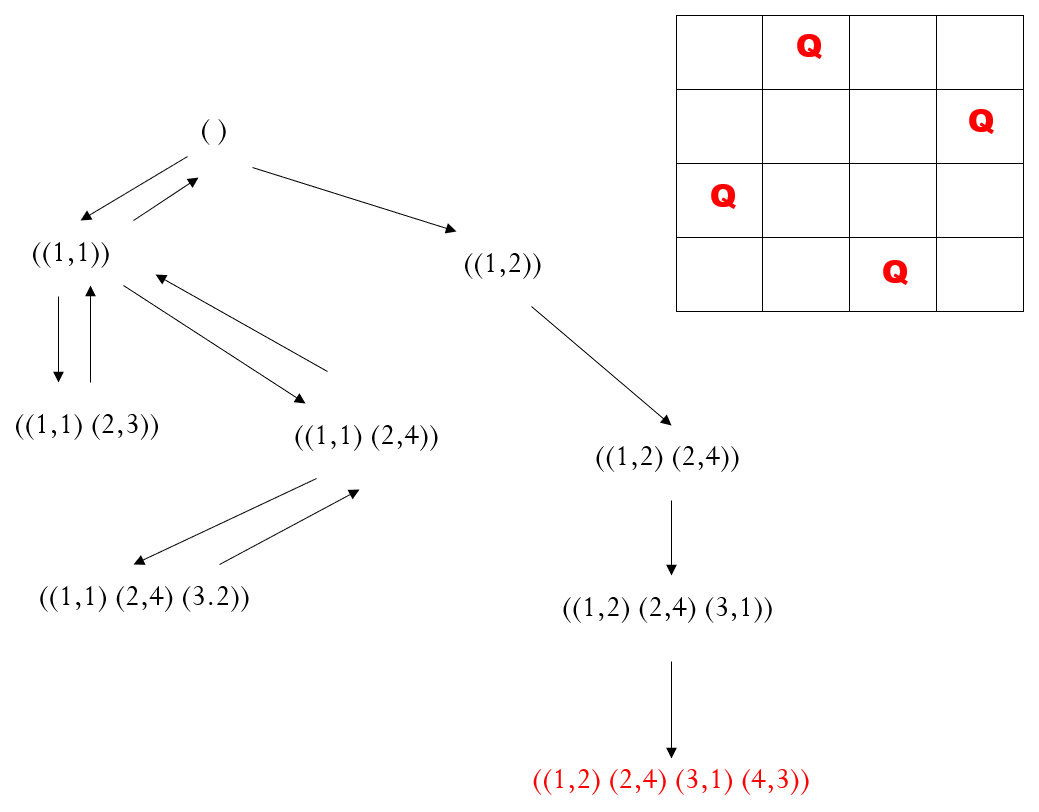
\includegraphics[width=0.95\linewidth]{figs/8-Queen.png}
%     % \caption{4-Queen Example.
%     % \vskip 10.1pt%
%     \label{fig:4-queen}
% \end{figurehere}

\textbf{深度优先搜索特点\ } 
\begin{itemize}
    \item 复杂度高,最坏情况退化为穷举
    \item 通用,与问题无关;但一般不保证找到最优解
    \item 节省内存,只存储初始节点到当前节点的路径
\end{itemize}

\subsection{宽度优先搜索}

\textbf{基本思路\ } 优先扩展深度浅的节点

\textbf{八数码问题\ }
规则:左上角开始顺时针 1-8
% (图)

% \begin{figurehere}
%     \centering    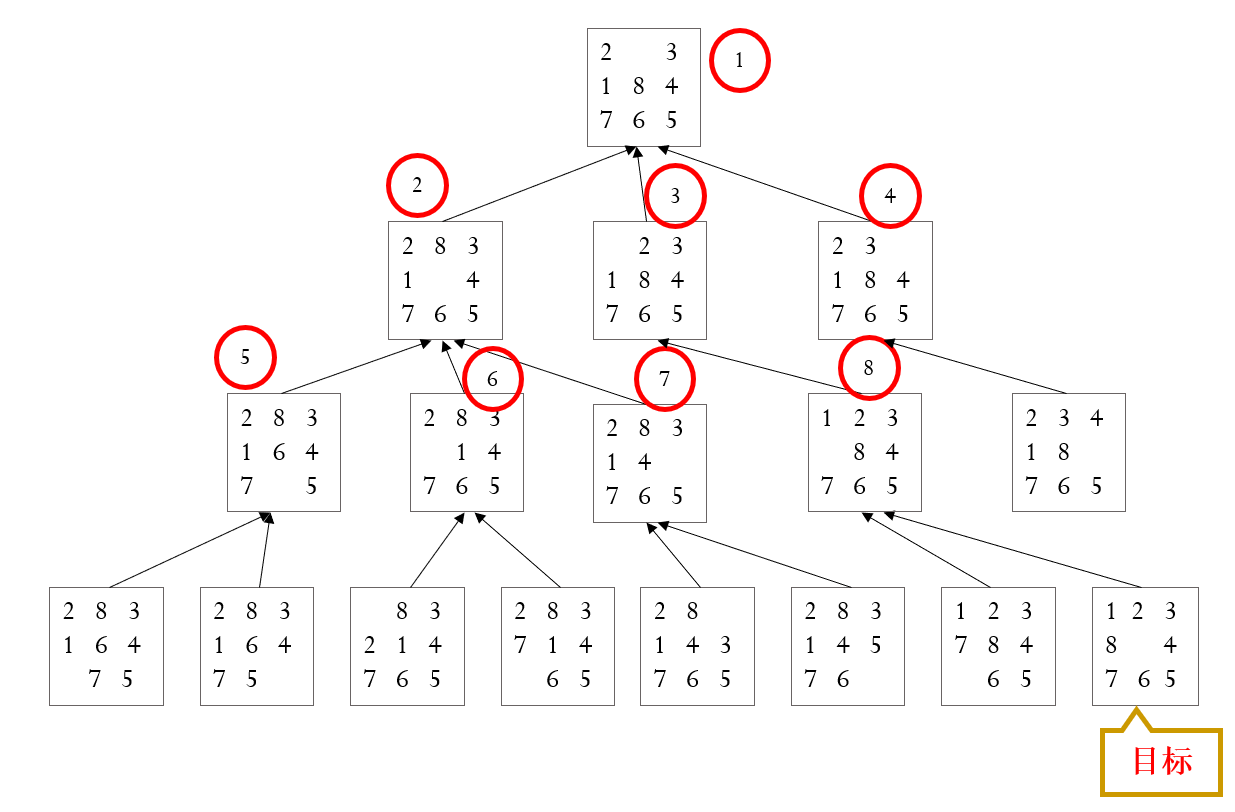
\includegraphics[width=0.95\linewidth]{figs/width-first.png}
%     % \caption{4-Queen Example.
%     % \vskip 10.1pt%
%     \label{fig:width-first}
% \end{figurehere}

\textbf{宽度优先搜索特点}
\begin{itemize}
    \item 问题有解时一定能找到解
    \item 当问题为单位耗散值时(且问题有解)时一定能找到最优解
    \item 方法通用,与问题无关;效率低,存储量大
\end{itemize}

\textbf{宽度优先搜索的不足\ } 未考虑两节点间的距离(权重)

\textbf{优化:迪杰斯特拉算法\ } 优先扩展距离起点最近的节点,直到终点距离最短

\begin{itemize}
    \item 优点:当问题有解时可以找到最优解
    \item 缺点:只考虑节点距离起点的距离,没考虑节点到终点的距离(单源单终点的目标场景)
\end{itemize}

\subsection{启发式图搜索}

引入启发知识,在保证找到最佳解的情况下,尽可能减少搜索范围,提高搜索效率。(核心是估计 h(n))

\textbf{启发知识\ } 评估节点到达目标的距离

\subsubsection{A算法}

\textbf{评价函数格式\ } f(n) = g(n) + h(n)
\begin{itemize}
    \item f(n):评价函数
    \item h(n):启发函数
\end{itemize}

% \textbf{符号}
\begin{itemize}
    \item g*(n):从s到n的最短路径的耗散值
    \item h*(n):从n到g的最短路径的耗散值
    \item f*(n)=g*(n)+h*(n):从s经过n到g的最短路径的耗散值
    \item g*(n),h*(n),f*(n)是不带*的估计值
    \item 用f(n)对待扩展节点进行评价
\end{itemize}

% (图)

\begin{figurehere}
    \centering    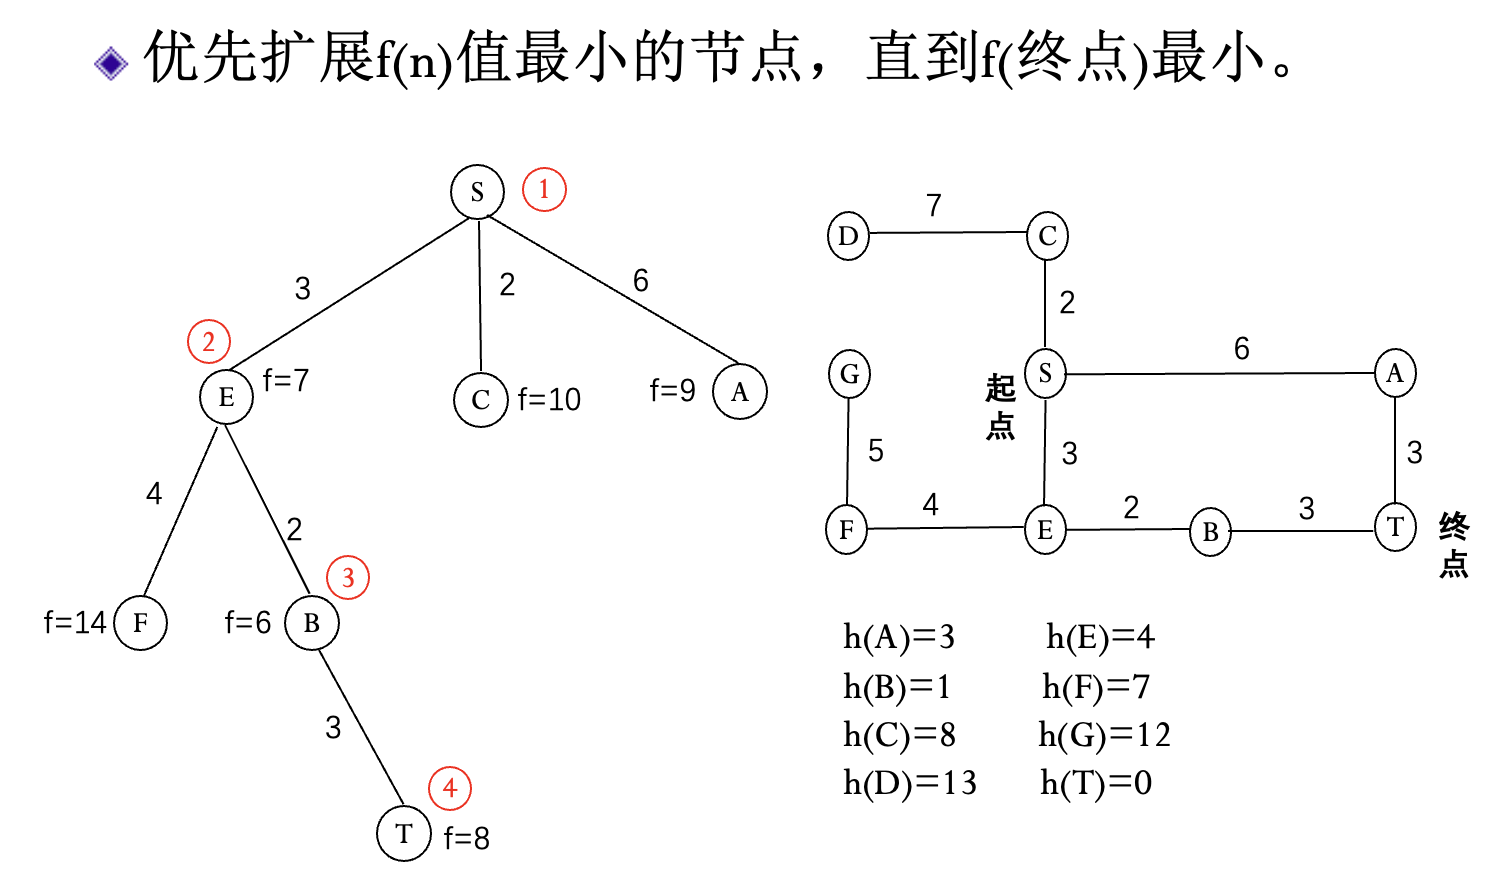
\includegraphics[width=0.9\linewidth]{figs/A-algo.png}
    % \caption{4-Queen Example.
    % \vskip 10.1pt%
    \label{fig:A-algo}
\end{figurehere}

\textbf{三类不同节点}
\begin{itemize}
    \item 新扩展生成节点 $m_j$
    \item 新扩展生成的节点先前已经生成过,但是子节点没有被扩展 $m_k$
    \item 新扩展生成的节点先前已经生成,子节点也已经扩展 $m_l$
\end{itemize}

\begin{lstlisting}[basicstyle=\tiny \ttfamily]
A-algorithm(s)   //s为初始节点
OPEN=(s), CLOSED=(), f(s)=g(s)+h(s);
while OPEN不空 do:
    begin
        n=FIRST(OPEN);
        if GOAL(n) THEN return n;
        REMOVE(n, OPEN), ADD(n, CLOSED);
        EXPAND(n) → {mi}, (生成所有子节点)
        计算f(n, mi)=g(n, mi)+h(mi);
        ADD(mj, OPEN), 标记mj到n的指针;
        if f(n, mk)<f(mk) then  // 如果新路小,则换指针
            f(mk)=f(n, mk), 标记mk到n的指针;
        if f(n, ml)<f(ml,) then // 新路小且有子节点,
                                   则要将该节点加入OPEN
            f(ml)=f(n, ml), 标记ml到n的指针, ADD(ml, OPEN);
        OPEN中的节点按f值从小到大排序;
    end while
return FAIL;

\end{lstlisting}

\textbf{八数码举例\ } 以“不在位牌数”为 h(n)

% (图)

% \begin{figurehere}
%     \centering    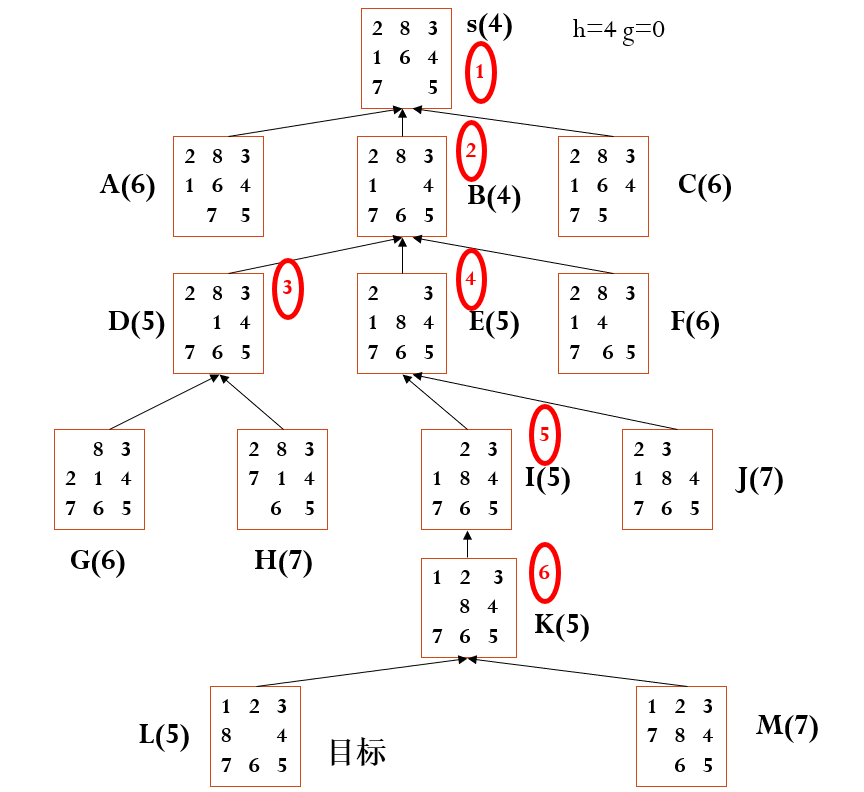
\includegraphics[width=0.95\linewidth]{figs/A-algo-8digits.png}
%     % \caption{4-Queen Example.
%     % \vskip 10.1pt%
%     \label{fig:A-algo-8d}
% \end{figurehere}

% \begin{figurehere}
%     \centering    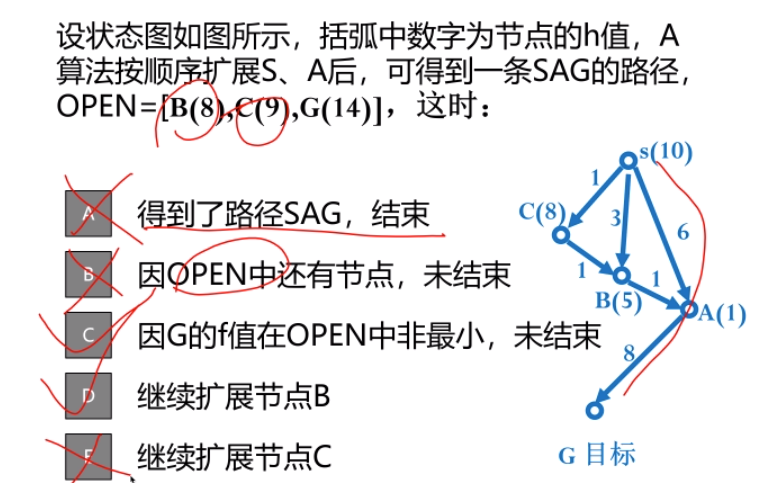
\includegraphics[width=0.95\linewidth]{figs/test1.png}
%     % \caption{4-Queen Example.
%     % \vskip 10.1pt%
%     \label{fig:A-algo-test}
% \end{figurehere}

\subsubsection{A*算法}

\textbf{A* 条件\ } 在 A 算法中满足条件 $h(n)\le h^*(n)$ 
% 则 A 算法称为 A* 算法。

% 例如八数码问题很容易证明,$h_1(n)$=“不在位”将排数是满足 A* 条件的;$h_2(n)$=“不在位”距离和也是满足 A* 条件的。需要具体问题具体分析。

\textbf{定义 h 函数的一般原则\ } 在\textbf{放宽的}限制条件下给出的估计函数一般都满足 A* 条件。

\textbf{传教士与野人的例子\ } M传教士C野人一次3人,左到右过河。任何地方野人不多于传教士。

简化假设只有乘船人数约束,假设船在左岸,则至少需要的摆渡次数:
$\lceil \frac{M+C-3}{2} \rceil \times 2 + 1 \ge M + C - 2$

如果船在右侧:M+C

综合:M+C-2b (船在左岸:b=0,右岸:b=1)

\textbf{A* 算法的两个主要结论}
\begin{itemize}
    \item 可采纳性定理:若存在从初始节点s到目标节点t的路径,则A*必然能找到最佳解
    \item 同一问题两个A*算法A1和A2,若A2比A1有更多启发信息,即 h2(n) > h1(n) (目标节点除外),则A1扩展的节点数 $\ge$ A2扩展的节点数(更精准的h函数不会让结果变差)
\end{itemize}

\textit{注意一个节点无论被扩展多少次都会只被计算一次}

\textit{考虑那些f(n)=f*(t)的节点,t为目标节点。如果不考虑这样的节点,\textbf{等号可以加上。}}

\textbf{h函数的评价方法\ } 平均分叉数

设一共扩展了 d 层节点,共搜索了 N 个节点,则 $N=(1-b*^{d+1})/(1-b*)$,b* 称为平均分叉数。

b* 越小说明 h函数的效果越好;实验表明,b* 比较稳定,同一问题基本不随问题规模变化。

\subsubsection{A* 算法的改进}
针对A算法中$m_l$类节点可能重新放回OPEN表导致重复扩展同一节点,搜索效率下降的问题。

\begin{figurehere}
    \centering    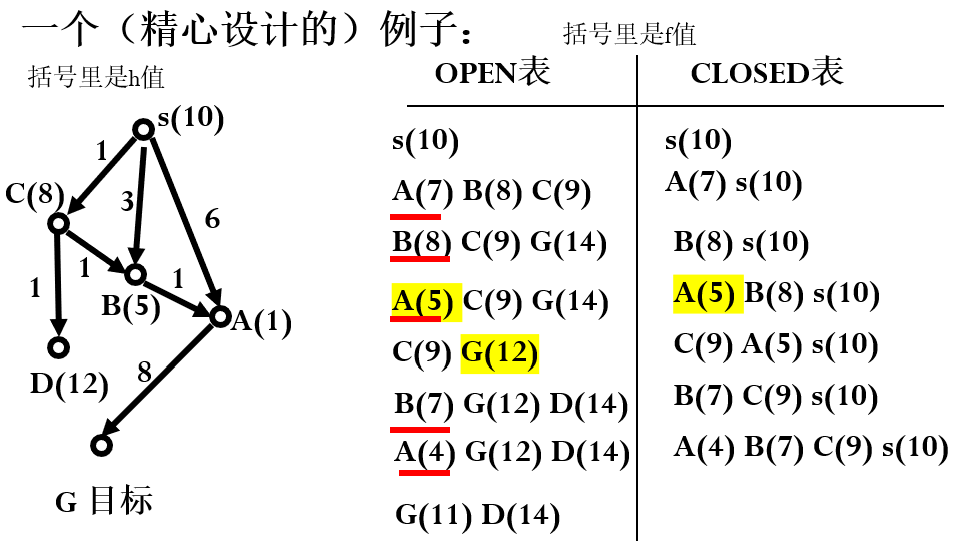
\includegraphics[width=0.95\linewidth]{figs/A-algo-shortest-path.png}
    % \caption{4-Queen Example.
    % \vskip 10.1pt%
    \label{fig:A-algo-sp}
\end{figurehere}

多次扩展的原因:前面并没有找到到A的最短路。

\textbf{改进方向}
\begin{itemize}
    \item 限制h函数,第一次扩展一个节点时就最短
    \item 改进算法,避免或减少多次扩展同一节点
\end{itemize}

\textbf{注意事项\ } 可采纳性、不多扩展、不增复杂性
% \begin{itemize}
%     \item 可采纳性不变
%     \item 不会多扩展节点
%     \item 不增加算法的复杂性
% \end{itemize}

% \newpage

\textbf{一种h改进方法\ } 设 $n_i$ 是 $n_j$ 的父节点,$C(n_i,n_j)$ 是二者间耗散值,$t$ 是目标,则合理的 h 函数应该满足 $h(n_j)\ge h(n_i)-C(n_i,n_j)$(或 $h(n_i) - h(n_j) \le C(n_i,n_j)$,$h(n_i)\le h(n_j)+C(n_i,n_j)$),且 $h(t)=0$,称此时的 h 函数是\textbf{单调的}。
(助记:三角不等式)

\textbf{定理\ } 若 h(n) 是单调的,则 A* 扩展了节点n之后,就已经找到了到达节点n的最佳路径

\textbf{推论\ } 满足单调的 h 一定满足 A* 条件。

\textbf{一种算法改进方法} 

% 结论:
\begin{itemize}
    \item OPEN 表上任何具有 $f(n)<f^*(s)$ 的节点一定会被 A* 扩展
    \item A*选作扩展的任一节点,定有 $f(n)\le f^*(s)$
    \item 当h(n)恒等于0时,h为单调的
\end{itemize}

改进思路:$f_m$ 初始为 0,后续赋值为目前已扩展节点最大 $f$ 值,用 $f_m$ 代替 $f^*(s)$,OPEN=(...f*(s)...),左边h设置为0,即不会重复扩展,右边不变。

\begin{lstlisting}[basicstyle=\tiny \ttfamily]
A-algorithm(s)   //s为初始节点
OPEN=(s), CLOSED=(), f(s)=g(s)+h(s);
while OPEN不空 do:
    begin
        NEST={ni|f(ni)<fm,ni 属于 OPEN}
        if NEST != () then n=NEST中g最小的节点 // 相当于h=0
        else n=FIRST(OPEN), fm=f(n);
        if GOAL(n) THEN return n;
        REMOVE(n, OPEN), ADD(n, CLOSED);
        EXPAND(n) → {mi}, (生成所有子节点)
        计算f(n, mi)=g(n, mi)+h(mi);
        ADD(mj, OPEN), 标记mj到n的指针;
        if f(n, mk)<f(mk) then  // 如果新路小,则换指针
            f(mk)=f(n, mk), 标记mk到n的指针;
        if f(n, ml)<f(ml,) then // 新路小且有子节点,
        则要加入OPEN
            f(ml)=f(n, ml), 标记ml到n的指针, ADD(ml, OPEN);
        OPEN中的节点按f值从小到大排序;
    end while
return FAIL;
\end{lstlisting}

\begin{figurehere}
    \centering    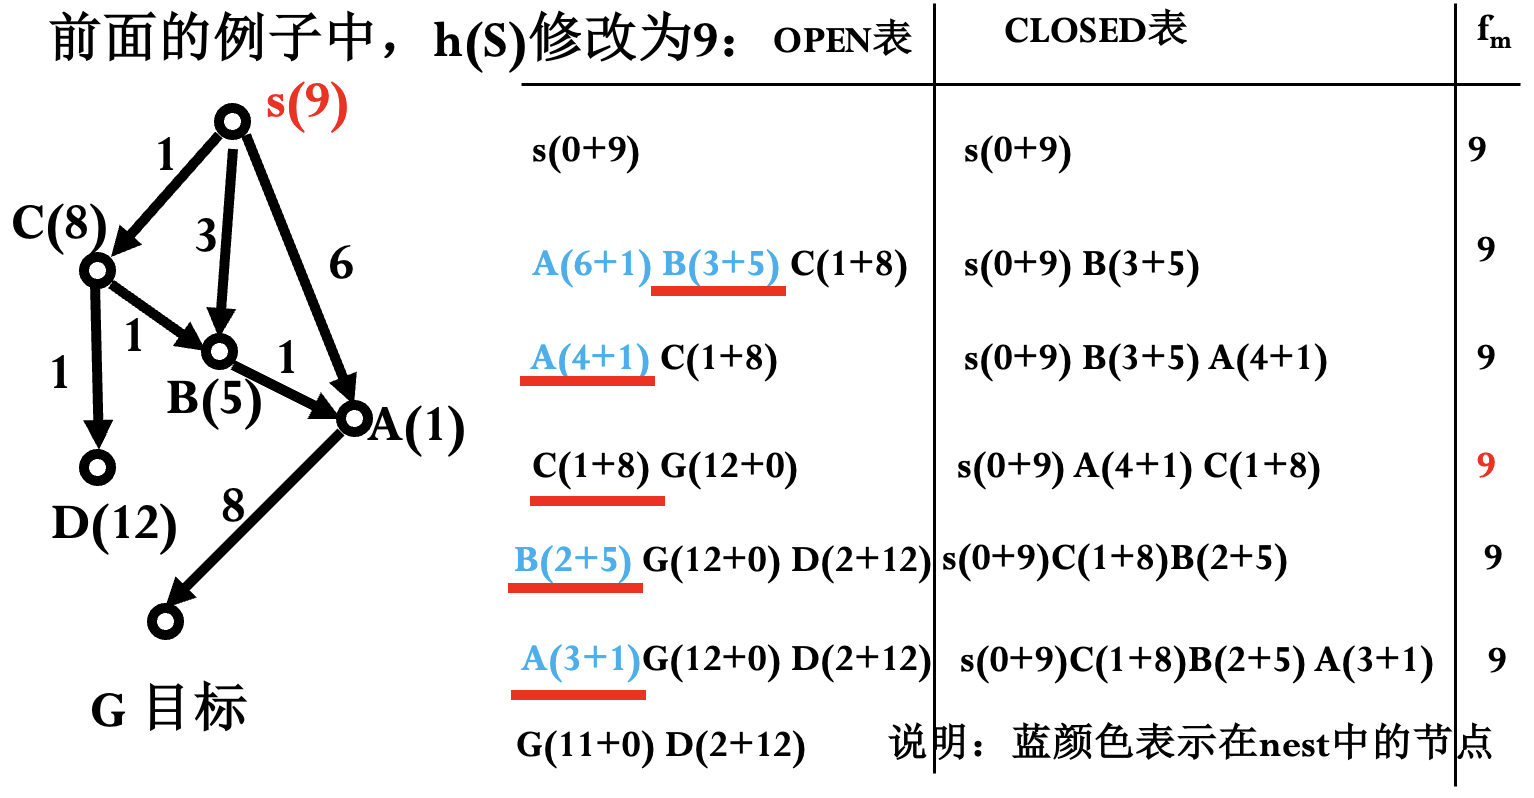
\includegraphics[width=0.95\linewidth]{figs/A-modified.png}
    % \caption{4-Queen Example.
    % \vskip 10.1pt%
    \label{fig:A-algo-modified}
\end{figurehere}

\subsection{其他的搜索方法}
\textbf{爬山法(局部搜索算法)\ } 要求全局光滑、单峰

% \textbf{随机搜索算法\ } 公众号第四篇

\textbf{动态规划算法\ }  h(n)=0 ,A* 算法 $\to$ 动态规划

\textbf{viterbi 算法\ } 按层找最短路径

$
Q(W_{i,j}) = 
\begin{cases}
\underset{k}{min}(Q(W_{i-1,k})+D(W_{i-1,k},W_{i,j}), i\ne 0\\
0,i=0
\end{cases}
$
其中:$Q(W_{i,j})$ 表示起点到点 $W_{i,j}$ 的最佳路径值; $D(W_{i-1,j}, W_{i,k})$ 表示 $W_{i-1,j}$ 到$W_{i,k}$ 的距离

\textbf{拼音输入法\ }

S:句子;O:拼音。
则拼音成句的概率:

\quad
$
P(S|O) = P(S)P(O|S)/P(O)
$

其中 $P(O)$ 是常量,$P(O|S)\approx 1$(句子对应的拼音基本是固定的)。因此转变为求 $P(S)$ 最大。

根据计算语言学中的统计语言模型:

\quad
$
P(S) = \Pi_{i=1}^n P(w_i|w_1\cdots w_{i-1})
$

问题:前面一串 $w_1\cdots w_{i-1}$ 的概率很难得到

简化:二元语法(任何一个字出现的概率只和前面一个字有关)
$
P(S) = \Pi_{i=1}^n P(w_i|w_{i-1})
$

上式取max等价于:
$
min\left(-\sum_{i=1}^n log(P(w_i|w_{i-1})\right)
$

概率的计算(语言模型)

\quad
$
P(w_i|w_{i-1})=\frac{w_{i-1}w_{i}\mbox{同时出现的次数}}{w_{i-1}\mbox{出现的次数}}
$

平滑处理:解决 $P(w_i|w_{i-1})$ 可能为0的问题,例如
$
P(w_i|w_{i-1}) = \lambda P(w_i|w_{i-1}) + (1-\lambda) P(w_i)
$

\textbf{汉字识别后处理\ } 
S:句子;O:待识别的句子图片。
则图片成句的概率:
$
P(S|O) = P(S)P(O|S)/P(O)
$

其中 $P(O)$ 是常量,$P(O|S)$ 用识别置信度 $CF(w_i$ 代替。问题转变为求
$\Pi_{i=1}^n P(w_i|w_{i-1})CF(w_i)$
最大。

\section{神经网络与深度学习}
\textbf{概念关系\ } 深度学习 $\subseteq$ 机器学习 $\subseteq$ 人工智能 

% \textbf{神经网络\ } 人工神经元网络(ANN、NN)

\subsection{初识神经网络——从数字识别谈起}
% \textbf{从图像识别模式匹配理解参数的作用}

% $net=w_1x_1+w_2x_2+\cdots+w_nx_n$
% 其中 $w_i\in \{1,-1\}$ 是数字模式;$x_i\in \{1,0\}$ 是数字图像。点乘结果大则匹配,结果小则不匹配。

% \textbf{引入激活函数 Sigmoid\ }
% 把结果变换到 0-1 之间

% $\sigma(net) = \frac{1}{1+e^{-net}}$

% \textbf{增加偏置}
% $\sigma(net+b)$

% \textbf{最终结果\ } $net=\sum w_ix_i+b, y=sigmoid(net)$

% 也就是一个神经元的基本表达式

% \textbf{神经网络的横向扩展\ } 增加模式

% \textbf{神经网络的纵向扩展\ } 局部模式识别

% \begin{figurehere}
%     \centering    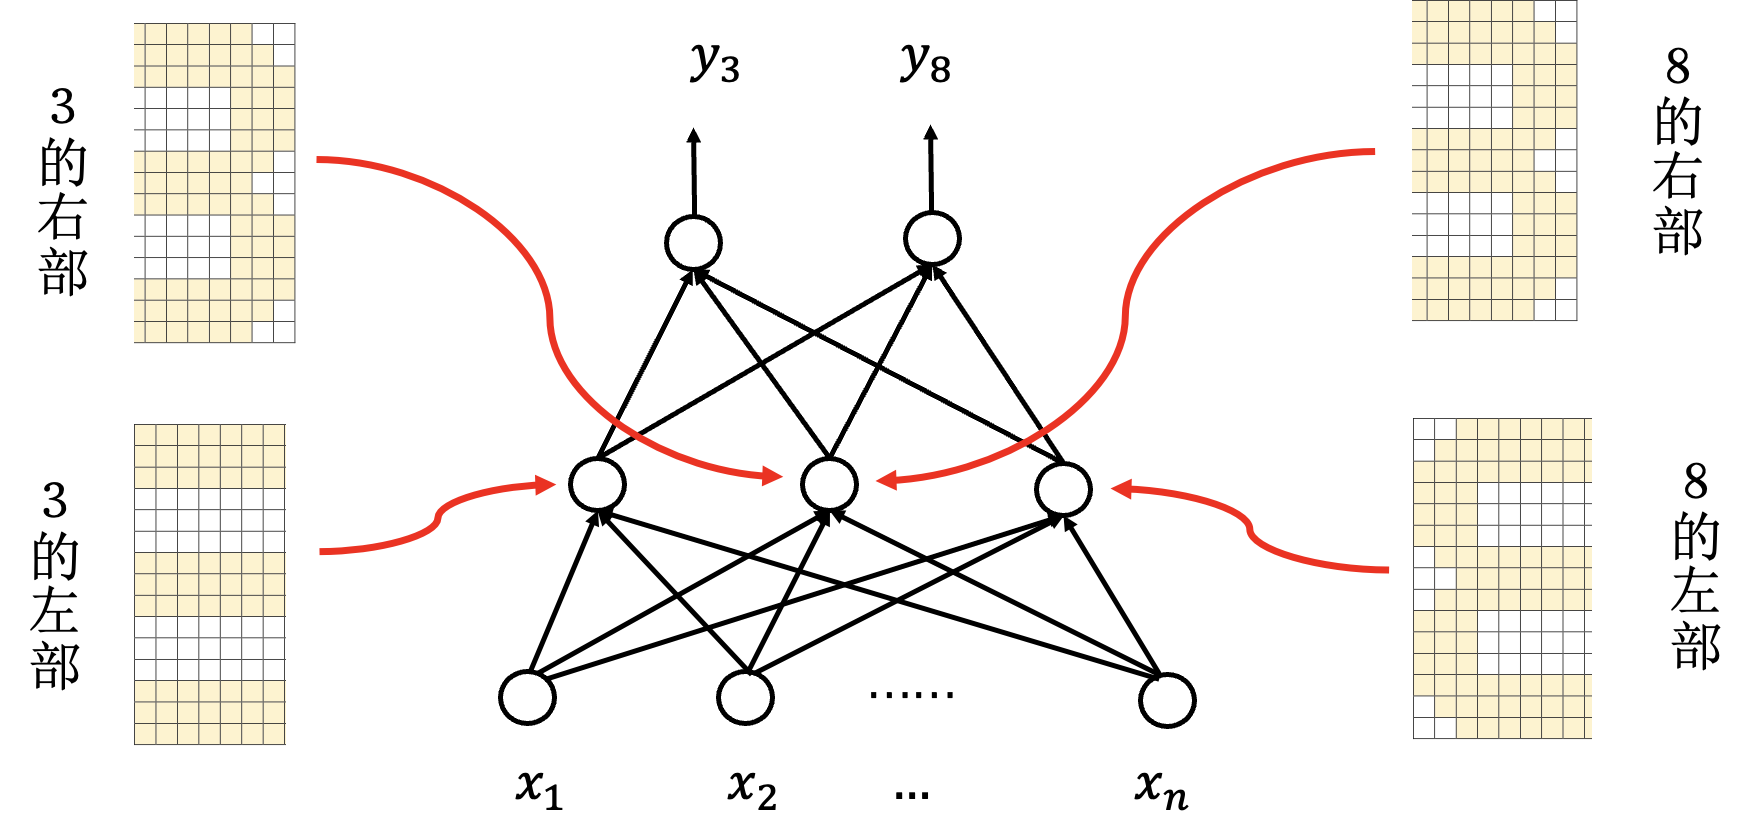
\includegraphics[width=0.95\linewidth]{figs/neuralnetwork38.png}
%     % \caption{4-Queen Example.
%     % \vskip 10.1pt%
%     \label{fig:nn38}
% \end{figurehere}

% 神经网络的深度变深→模式细化
% 输入层→隐含层→ 输出层

% \textbf{模式的获得\ } 通过训练样本自动学习权重,即模式;学习到的模式是一种隐含的表达  

% \rule{0.33\textwidth}{0.4pt}
\subsection{神经元与神经网络}
\textbf{神经元\ }
令$x_0=1, w_0=b$,则

$net = \sum_{i=0}^n w_ix_i=w\cdot x$

\textbf{常见激活函数}
\begin{itemize}
    \item 符号函数:$sgn(net)=net\ge 0?1:-1$
    \item Sigmoid: $\sigma(net) = \frac{1}{1+e^{-net}}$ 求导方便
    \item 双曲正切:$tanh(net)=\frac{e^{net}-e^{-net}}{e^{net}+e^{-net}}$
    \item 线性整流函数:$ReLU(net)=max(0,net)$
    \item Softmax:$o_k=\frac{e^{net}k}{\sum_{i=1}^m e^{net}i}$ 
    作用在整个一层上。

    性质:$0\le o_k\le 1, \sum_{k=1}^m o_k=1$,可当概率用
\end{itemize}

\textbf{全连接网络(Fully-Connected Network)}

也称前馈网络,多层感知机,全连接层,稠密层

\subsection{神经网络的训练}

\textbf{建立数据集\ } 收集多种数据、数据标注、数据集划分

\textbf{损失函数\ } 误差平方和

样本 d 的误差: $E_d(w)=\frac{1}{2} \sum_{k=1}^m (t_{kd}-o_{kd})^2$

所有样本的误差: $\frac{1}{2} \sum_{d=1}^n E_d(w)$

$t_{kd}$:对应样本d的第k个希望输出

$o_{kd}$:对应样本d的第k个实际输出

\textbf{梯度下降法\ } $w_{i}^{new} = w_i^{old}+\Delta w_i, \Delta w_i = -\eta \frac{\partial E(w)}{\partial w_i}$

\textbf{梯度下降算法}
\begin{itemize}
    \item 批量梯度下降算法(batch): 每次全部样本,慢
    \item 随机梯度下降算法 (SGD): 噪声敏感
    \item 小批量梯度下降算法 (mini-batch): 折中多用
\end{itemize}

\textbf{Back Propagation (BP)——反向传播算法}

\textbf{梯度计算——输出层\ } 

$\frac{\partial E_d}{\partial w_{ji}} = \frac{\partial E_d}{\partial net_j}\cdot \frac{\partial net_j}{\partial w_{ji}}$
:
$\frac{\partial E_d}{\partial net_j}=\frac{\partial E_d}{\partial o_j} \cdot \frac{\partial}{\partial net_j}$, $\frac{\partial net_j}{\partial w_{ji}}=x_{ji}$,
$\frac{\partial E_d}{\partial o_j} = -(t_j-o_j)$, $\frac{\partial o_j}{\partial net_j} = \frac{\partial \sigma}{\partial net_j} = o_j(1-o_j)$.

令 $\delta_j=-\frac{\partial E_d}{\partial net_j}=(t_j-o_j)o_j(1-o_j)$

则 $\frac{\partial E_d}{\partial w_{ji}} = -\delta_j x_{ji}$

\textbf{梯度计算——隐含层\ }

$\frac{\partial E_d}{\partial w_{ji}} = \frac{\partial E_d}{\partial net_j} \cdot \frac{\partial net_j}{\partial w_{ji}}$, $\frac{\partial net_j}{\partial w_{ji}} = x_{ji}$

$\frac{\partial E_d}{\partial net_j} = \underset{k\in \small{\mbox{后继}}(j)}{\sum} \frac{\partial E_d}{\partial net_k} \cdot \frac{\partial net_k}{\partial net_j} = -\underset{k\in \small{\mbox{后继}(j)}}{\sum} \delta_k \cdot \frac{\partial net_k}{\partial net_j}$

$\frac{\partial net_k}{\partial net_j} = \frac{\partial net_k}{\partial o_j} \cdot \frac{\partial o_j}{\partial net_j}$, $\frac{\partial net_k}{\partial o_j} = w_{kj}$, 

$\frac{\partial o_j}{\partial net_j} = o_j(1-o_j)$

令 $\delta_j = -\frac{\partial E_d}{\partial net_j} = o_j(1-o_j) \underset{k\in \small{\mbox{后继}}(j)}{\sum} \delta_k \cdot w_{kj}$

则 $\frac{\partial E_d}{\partial w_{ji}} = -\delta_j x_{ji}$

以此类推:$\Delta w_{ji} = -\eta \frac{\partial E_d}{\partial w_{ji}} = \eta \delta_j x_{ji}$,$\eta$ 是步长

\begin{figurehere}
    \centering    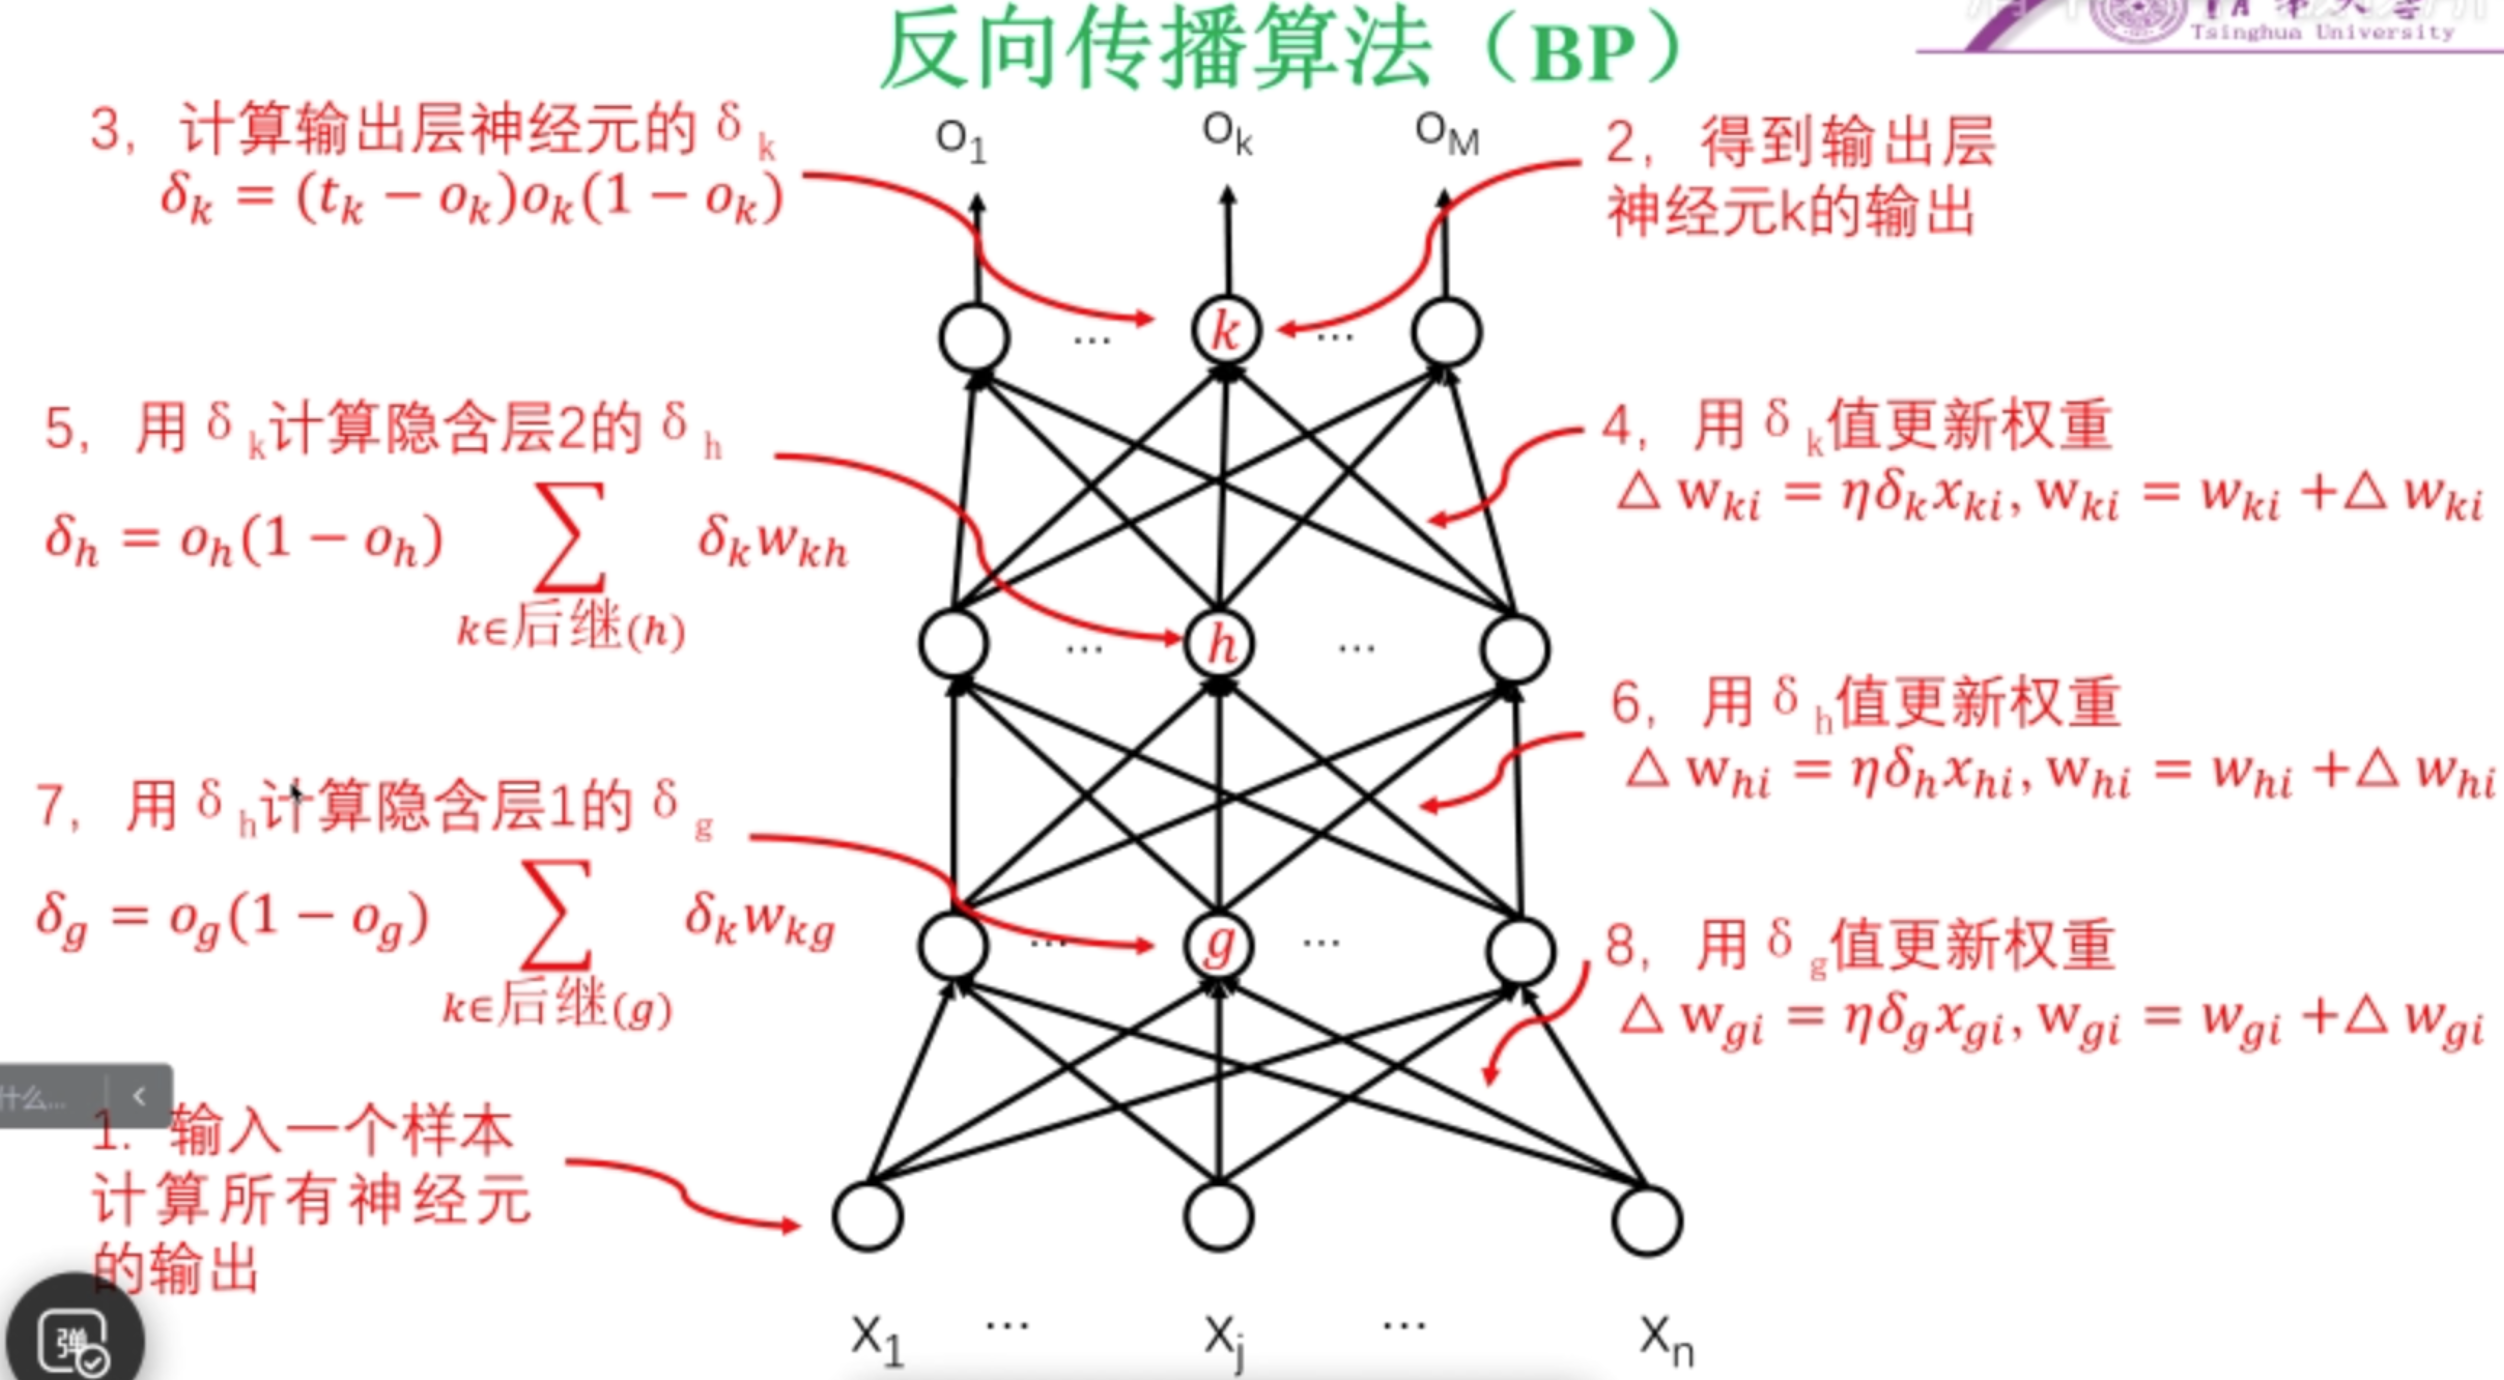
\includegraphics[width=0.95\linewidth]{figs/BP.png}
    % \caption{4-Queen Example.
    % \vskip 10.1pt%
    \label{fig:BP}
\end{figurehere}

\textbf{随机梯度下降的BP\ } 初始化所有权值为小随机

\textbf{该 BP 算法条件\ } 

全连接、随机梯度、Sigmoid、误差平方和

\textbf{交叉熵损失函数\ } (画图感受会非常直观)

$H_d(w)=-\sum_{k=1}^M t_{kd} log(o_{kd})$, 

$H(w) = \sum_{d=1}^N H_d(w) = -\sum_{d=1}^N\sum_{k=1}^M t_{kd} log(o_{kd})$

$t_{kd}$:样本d对应的希望输出值

$o_{kd}$:样本d对应的实际输出值,要求是个概率值

注意事项:
\begin{itemize}
    \item 一般先用 softmax 转换为概率
    \item 对于\textbf{分类问题}(只有一个目标值为1,其他为0),可简化为 $H_d(w) = -log(o_{kd})$,\textbf{特别有用}
\end{itemize}

\textbf{两种损失函数及作用}
\begin{itemize}
    \item 误差平方和:输出具体数值
    \item 交叉熵损失函数:用于分类问题
\end{itemize}

\subsection{卷积神经网络CNN}
\textbf{全连接神经网络的不足\ } 

连接权重过多、影响训练速度、影响使用速度
% \begin{itemize}
%     \item 连接权重过多
%     \item 影响训练速度
%     \item 影响使用速度
% \end{itemize}

% \textbf{提出背景\ } 是否可以提取局部模式

\textbf{卷积神经网络特点\ } 局部连接、权值共享

\textbf{举例\ } 边缘提取

\textbf{卷积核大小\ } 一般是奇数 $3\times 3, 5\times 5, 7\times 7$

\textbf{填充\ } 卷积之后外围填充,保持维数不变

\textbf{步长\ } 卷积核每次移动的距离

\textbf{多卷积核\ } 一个卷积核产生一个通道→多通道

\textbf{多通道输入\ } 每个输入通道有一个卷积核,\textbf{输出为一个通道}(多输入通道的多层卷积核结果加在一起)

\textbf{卷积核大小\ } 小卷积核:细粒度;大卷积核:粗粒度

多层小卷积实现大卷积 (例如2*(3*3)等效(5*5))

\textbf{做题易错提醒\ } 注意不要遗漏\textbf{偏置}!

\textbf{池化\ } 一种降维手段(稀疏但保留主要特征)

窗口和步长可以设定
\begin{itemize}
    \item 最大池化:取窗口中的最大值
    \item 平均池化:取窗口中的平均值
\end{itemize}

池化作用在单个通道上,不改变通道数目

\textbf{神经网络应用举例}

\textbf{LeNet 神经网络\ }

\begin{figurehere}
    \centering    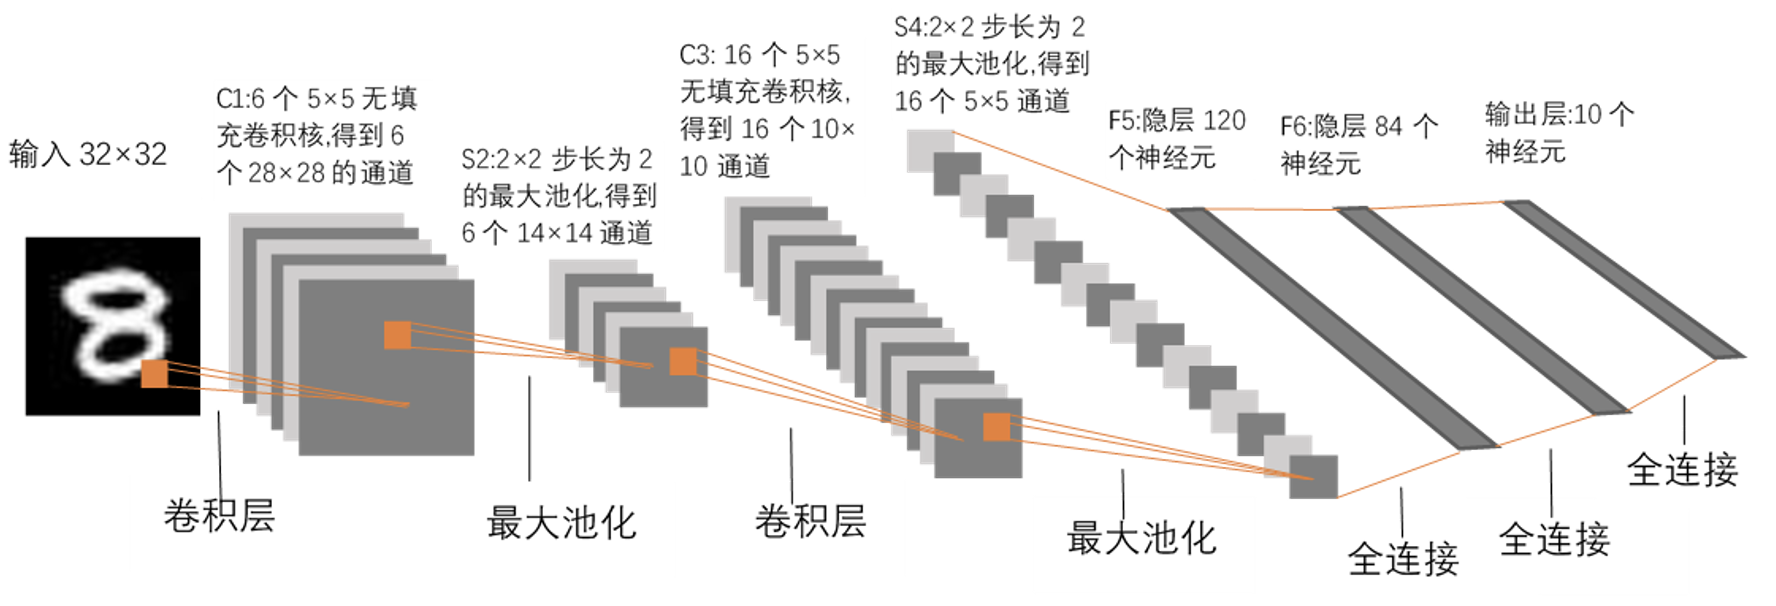
\includegraphics[width=0.95\linewidth]{figs/LeNet.png}
    % \caption{4-Queen Example.
    % \vskip 10.1pt%
    \label{fig:LeNet}
\end{figurehere}

注意:C3 的 16 个卷积核每个厚度默认是 6;S4→F5 可以直接展开 16 个通道,与后面做全连接即可

\textbf{VGG-16}

\begin{figurehere}
    \centering    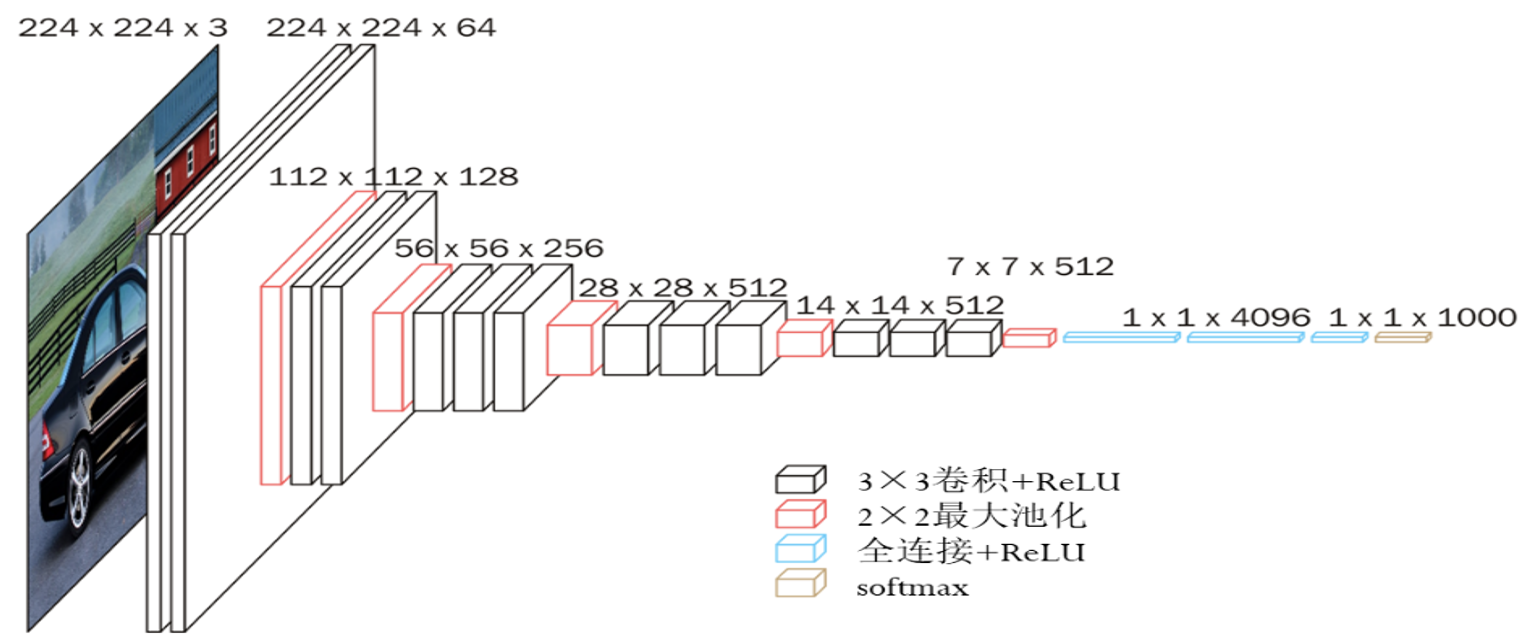
\includegraphics[width=0.95\linewidth]{figs/VGG-16.png}
    % \caption{4-Queen Example.
    % \vskip 10.1pt%
    \label{fig:LeNet}
\end{figurehere}

注意:此处有填充

参数计算举例:224*224*64两层之间的参数量

\quad $3\times 3\times 64\times 64+64=36928$

\textbf{CNN 可解释性\ } 卷积核具有抽取特征的能力

\textbf{CNN 的特点\ } 
\begin{itemize}
    \item 参数量少,只与卷积核的大小和数量相关
    \item 具有特征抽取能力
    \item 特征具有一定程度上的平移不变性
\end{itemize}

\subsection{梯度消失问题}

\textbf{梯度消失问题来源\ } 若使用 Sigmoid 激活函数,有如下梯度关系
$\delta_j = o_j(1-o_j) \underset{\sum}{k\in \small{\mbox{后继}}(j)} \delta_k w_{kj}$

其中 $o_j(1-o_j) \le 0.25$,因此当网络层数增多$\delta_j \to 0$

梯度消失:$\Delta w_{ji} = \eta \delta_j x_{ji} \to 0$

\textbf{一种解决方案\ } 使用 ReLU 等激活函数。

\textbf{GoogLeNet\ } 
\begin{itemize}
    \item 基于 Inception 模块的组合:并联多个不同大小的卷积核(有填充),可以同时抽取不同粒度的特征,并结合输入的“最明显特征”(最大池化);可进一步加入1*1卷积核降维处理
    \item 引入辅助 Softmax 缓解梯度消失问题\\ 辅助输出:平均池化+卷积层+全连接*2+softmax;可实现部分参数更新,层层下推
\end{itemize}

\begin{figurehere}
    \centering    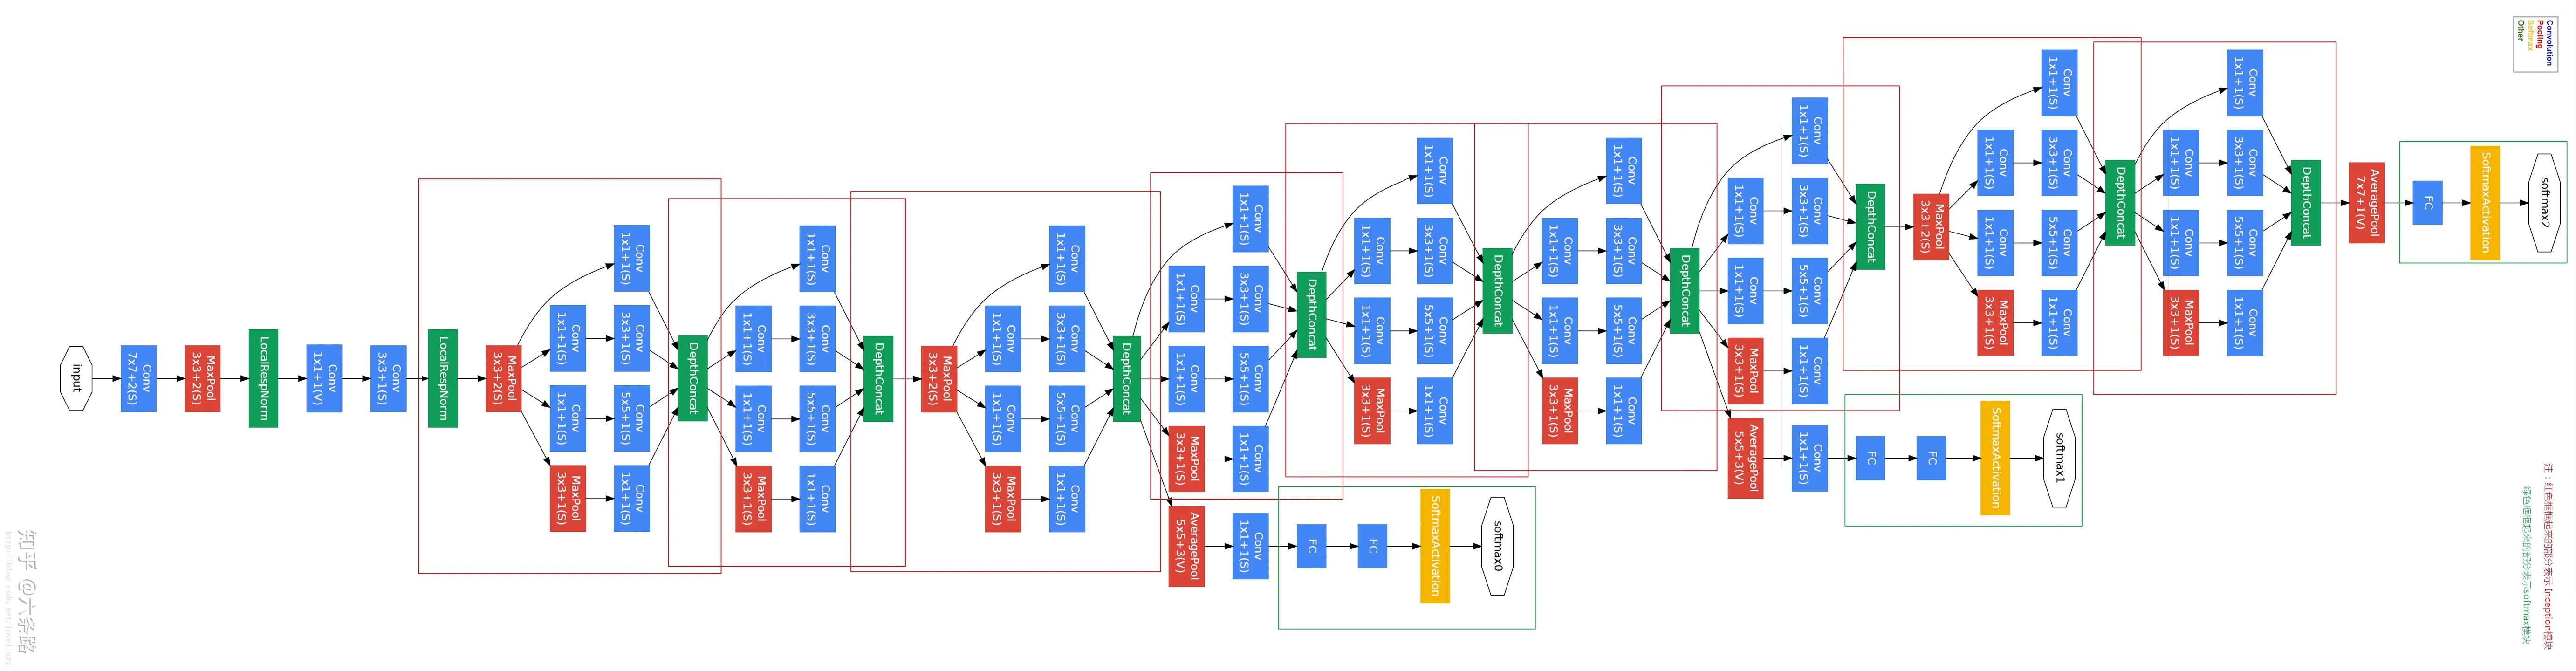
\includegraphics[width=0.95\linewidth]{figs/Googlenet.png}
    % \caption{4-Queen Example.
    % \vskip 10.1pt%
    \label{fig:GoogLeNet}
\end{figurehere}

\textbf{ResNet 残差网络\ }  

核心思想:$F'(x) = F(x) + x$ (残差模块、恒等映射,注意通道数、通道大小必须一致)

\begin{figurehere}
    \centering    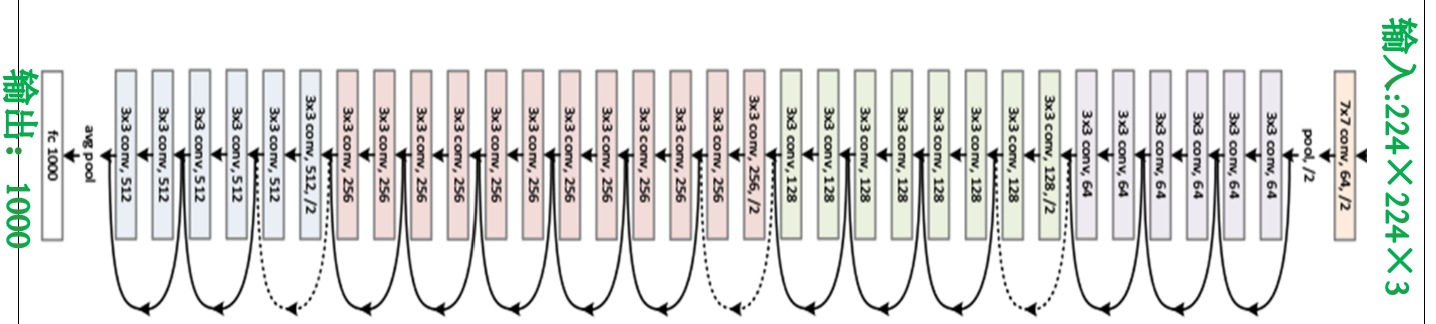
\includegraphics[width=0.95\linewidth]{figs/ResNet.png}
    % \caption{4-Queen Example.
    % \vskip 10.1pt%
    \label{fig:ResNet}
\end{figurehere}

其中虚线部分恒等映射需要等维处理(比如用合适的卷积,并使用合适的步长)

全局平均池化:一个平面变成一个值

\textbf{稠密网络\ } 网上多层连接,但参数更少,性能更好

\subsection{过拟合问题}
\textbf{减少过拟合的方法\ }
\begin{itemize}
    \item \textbf{使用验证集}:验证集错误率最低时停止\\
    注意若不区分验证集测试集,测试结果偏好
    \item \textbf{正则化项法}:例如误差平方和损失函数 + 2-范数
    $E_d(w) = \sum_{k=1}^M(t_{kd}-o_{kd})^2 + ||w||^2_2$\\ 其中 $||w||^2 = w_1^2+w_2^2+ \dots + w_N^2$\\
    \small{正则化项可以降低模型复杂性,即高次项系数$\to 0$}
    \item \textbf{舍弃法(dropout)}:随机临时舍弃一些神经元
    \item \textbf{数据增强 }:数据越多,过拟合风险越小\\ 数据增强方法:通过各种变换增加数据数量等
\end{itemize}

% \subsection{深度学习框架及神经网络应用}
% \textbf{框架\ } TensorFlow,Pytorch,PaddlePaddle
% \textbf{应用\ } 确认输入输出关系、收集样本、设计网络结构、设计损失函数、框架实现、超参数选择、调整试错。注意关注发展动态!



\section{对抗搜索}
\textbf{博弈问题\ } 双人、一人一步、双方信息完备、零和
\subsection{穷举问题}
对于象棋、围棋这类的棋类问题,穷举不可行
\subsection{极小-极大模型}
\textbf{基本思路\ } 
\begin{itemize}
    \item 向后看若干步(一定深度内穷举)
    \item 从最不利的情景中选择最有利的走法(即我方走取极大,对方走取我方极小,这样可以在对方“最聪明”的情况下把损失降到最低)
\end{itemize}

\textbf{缺点\ } 即便限定深度也无法穷举;有明显无效搜索 

\subsection{$\alpha - \beta $ 剪枝模型}
50年代麦卡锡就提出 $\alpha-\beta$ 剪枝算法

\textbf{算法原理\ } 有剪枝的深度优先搜索 
\begin{itemize}
    \item 极大节点的下界为 $\alpha$
    \item 极小节点的上界为 $\beta$
\end{itemize}

\textbf{剪枝的条件\ }(\textbf{注意 } 相等的时候也剪枝)
\begin{itemize}
    \item[1] 后辈节点的 $\beta$ 值 $\le$ 祖先节点的 $\alpha$ 值时\\ $\alpha$ 剪枝(极小 $\le$ 极大,剪枝)
    \item[2] 后辈节点的 $\alpha$ 值 $\ge$ 祖先节点的 $\beta$ 值时\\ $\beta$ 剪枝(极大 $\ge$ 极小,剪枝)
\end{itemize}


\textbf{理解\ } “我方”不会选择分数更低的,所以1;“对方” 不会选择(让“我方”)分数更高的,所以2

\begin{figurehere}
    \centering    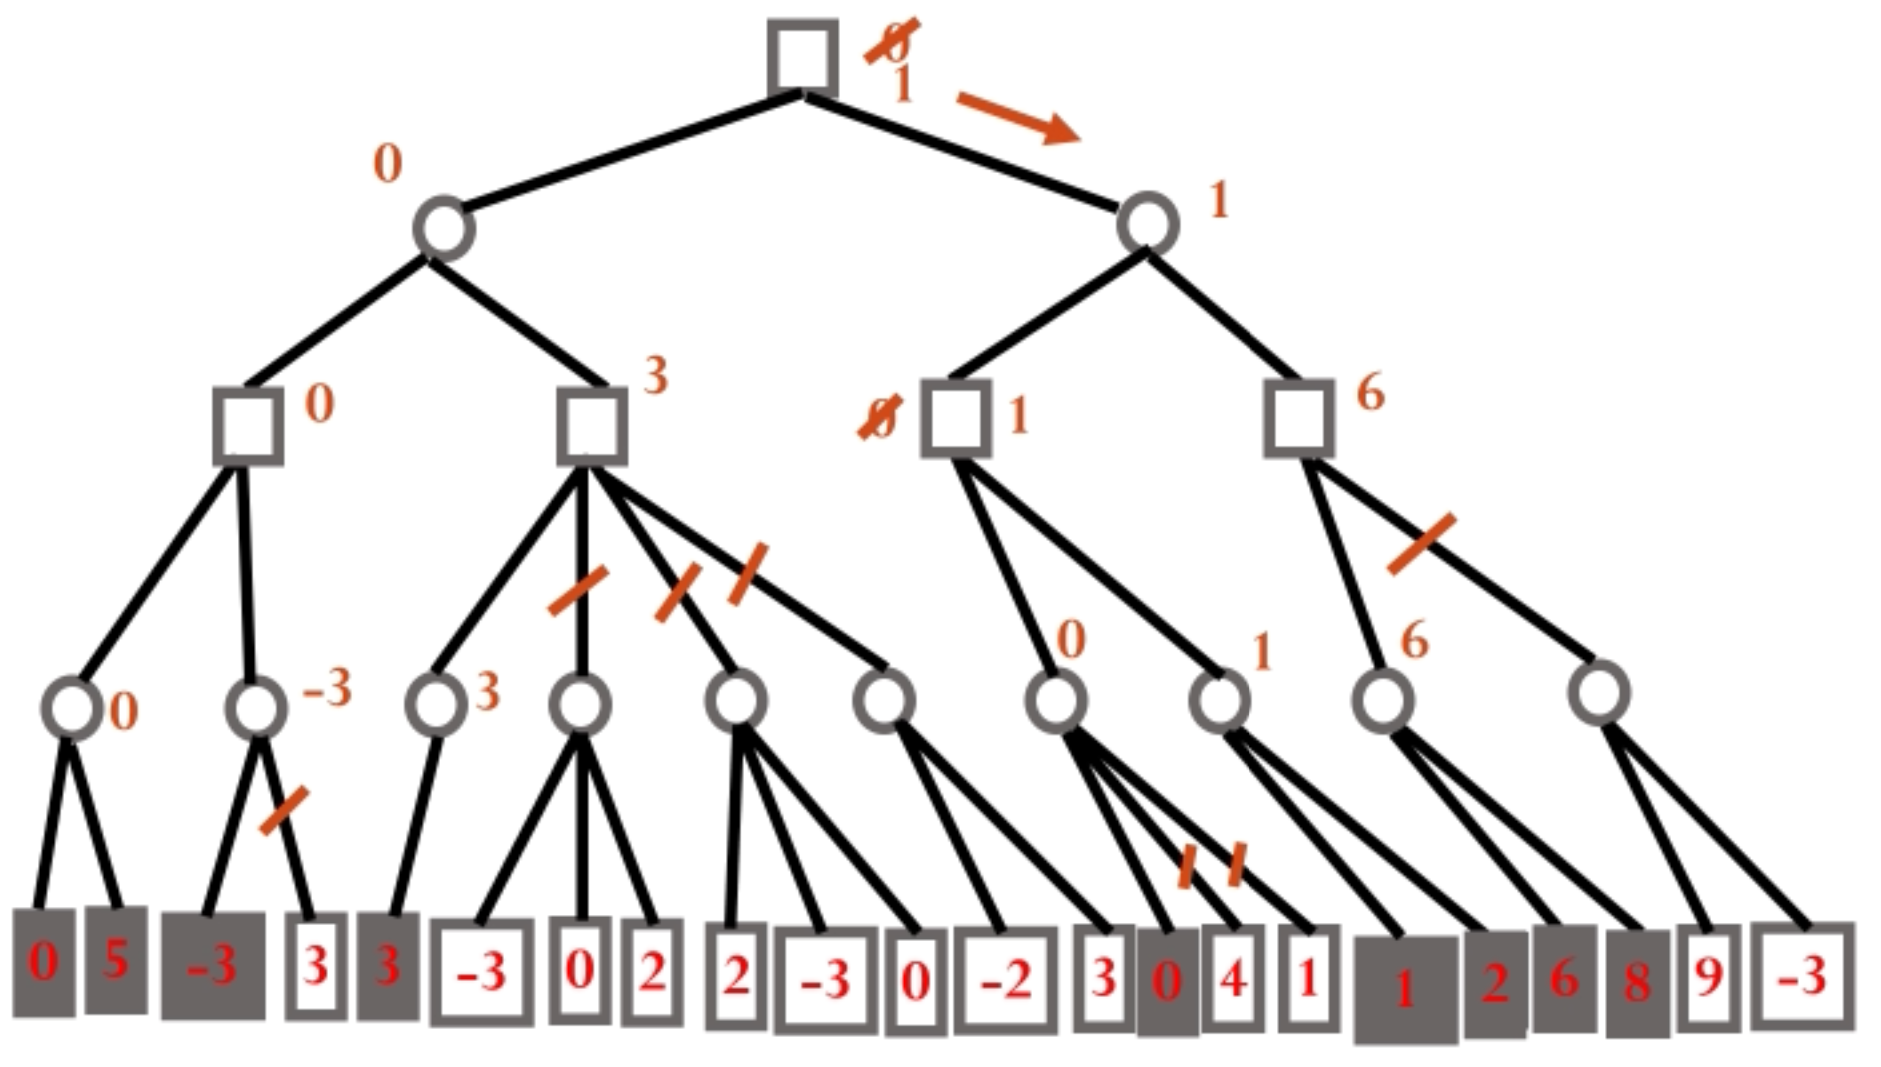
\includegraphics[width=0.9\linewidth]{figs/alpha-beta.png}
    % \caption{4-Queen Example.
    % \vskip 10.1pt%
    \label{fig:alpha-beta}
\end{figurehere}

从左到右,从下到上

注意考虑所有的“祖先”而不只是“父节点”

注意不要漏“剪”,极小极大都要考虑

注意最终只会得到“一步”结果,而不是直接到底

\textbf{回溯时机\ } 节点该扩展的扩展了,该剪枝的剪枝了,就可以回溯赋值(更新)父节点了

\textbf{如何估值\ } 总结专家知识进行估值

\textbf{算法的问题\ } 依赖于局面评估的准确性,需要大量专家知识或者知识统一性问题;在围棋上失效

\subsection{蒙特卡洛方法}
\textbf{基本思想\ } 从当前局面中所有可落子的点中随机选择一个点落子,重复上述过程直到胜负可判断,多次模拟之后选择胜率最大的点落子

\textbf{蒙特卡洛树搜索\ } 选择→扩展→模拟→回传

\textbf{选择策略\ }
\begin{itemize}
    \item 利用当前希望较大的节点(先验)
    \item 探索尚未充分了解的节点(检验)
\end{itemize}

\textbf{多臂老虎机模型\ } k 个拉杆,每个拉杆有概率收益且互不相关→寻找策略使拉动拉杆所获收益最大

\begin{lstlisting}[basicstyle=\tiny \ttfamily]
function UCB1
    for each 拉杆j:
        访问该拉杆并记录收益
    end for
    while 尚未达到访问次数限制 do:
        计算每个拉杆的UCB1信心上界Ij
        访问信心上界最大的手臂
    end while
\end{lstlisting}
$
I_j = \bar{X}_j+c\sqrt{\frac{2ln(n)}{T_j(n)}}
$
其中:$\bar{X}_j$ 是拉杆 $j$ 获得回报的均值;$n$ 是迄今为止访问的总次数;$T_j(n)$ 是拉杆 $j$ 到目前为止所访问的次数;$c$ 是调节参数

% 直观理解:“已有效果”和“探索”之间的平衡,即收益好、模拟次数少的优先选择

\textbf{信心上限树UCT算法}

% https://www.pianshen.com/article/2533458636/
% https://blog.csdn.net/newlw/article/details/126942737

\begin{figurehere}
    \centering    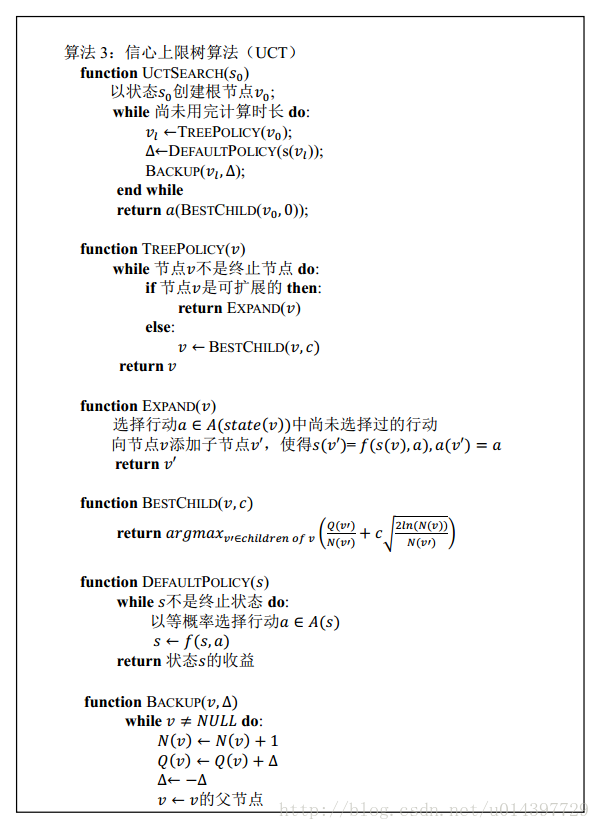
\includegraphics[width=0.95\linewidth]{figs/UCT.png}
    % \caption{4-Queen Example.
    \vskip -10pt
    \label{fig:UCT}
\end{figurehere}

每一次观察获胜次数是从“当前节点”角度出发的,即每一层分别是我方和对方获胜概率,类比上面的极小极大模型思路

% \begin{itemize}
%     \item 老师PPT只给了第一部分算法轮廓
%     \item 每一次观察获胜次数是从“当前节点”角度出发的,即每一层分别是我方和对方获胜概率,类比上面的极小极大模型思路
% \end{itemize}

\subsection{AlphaGo 原理}
\textbf{蒙特卡洛树存在的问题\ } 搜索盲目,没有围棋知识
% \begin{itemize}
%     \item 生成所有子节点
%     \item 搜索盲目,没有引入围棋知识
% \end{itemize}

\textbf{AlphaGo 原理\ } 将神经网络与蒙特卡洛树结合在一起;缩小了搜索范围,提高了模拟水平

\textbf{如何引入专家知识\ } 把围棋类比成分类任务,16万盘棋谱,任意一个棋局分类为361(19*19)类之一

\textbf{AlphaGo 使用的两类网络}
\begin{itemize}
    \item 策略网络(Rollout快速网络、SL、RL)
    \item 估值网络
\end{itemize}

\begin{figurehere}
    \centering    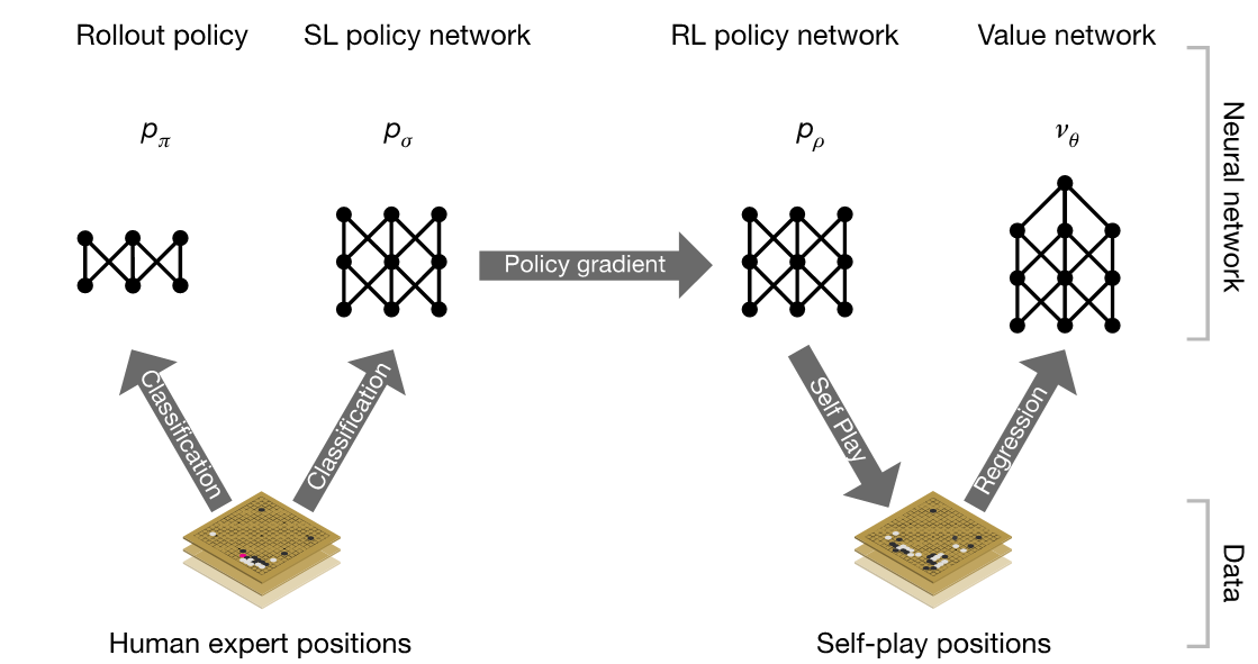
\includegraphics[width=0.95\linewidth]{figs/AlphaGo-2.png}
    % \caption{4-Queen Example.
    % \vskip 10.1pt%
    \label{fig:AlphaGo-2}
\end{figurehere}

\textbf{策略网络\ } 神经网络

输入:当前棋局,48*19*19

输出:在每个点落子的概率

\begin{figurehere}
    \centering    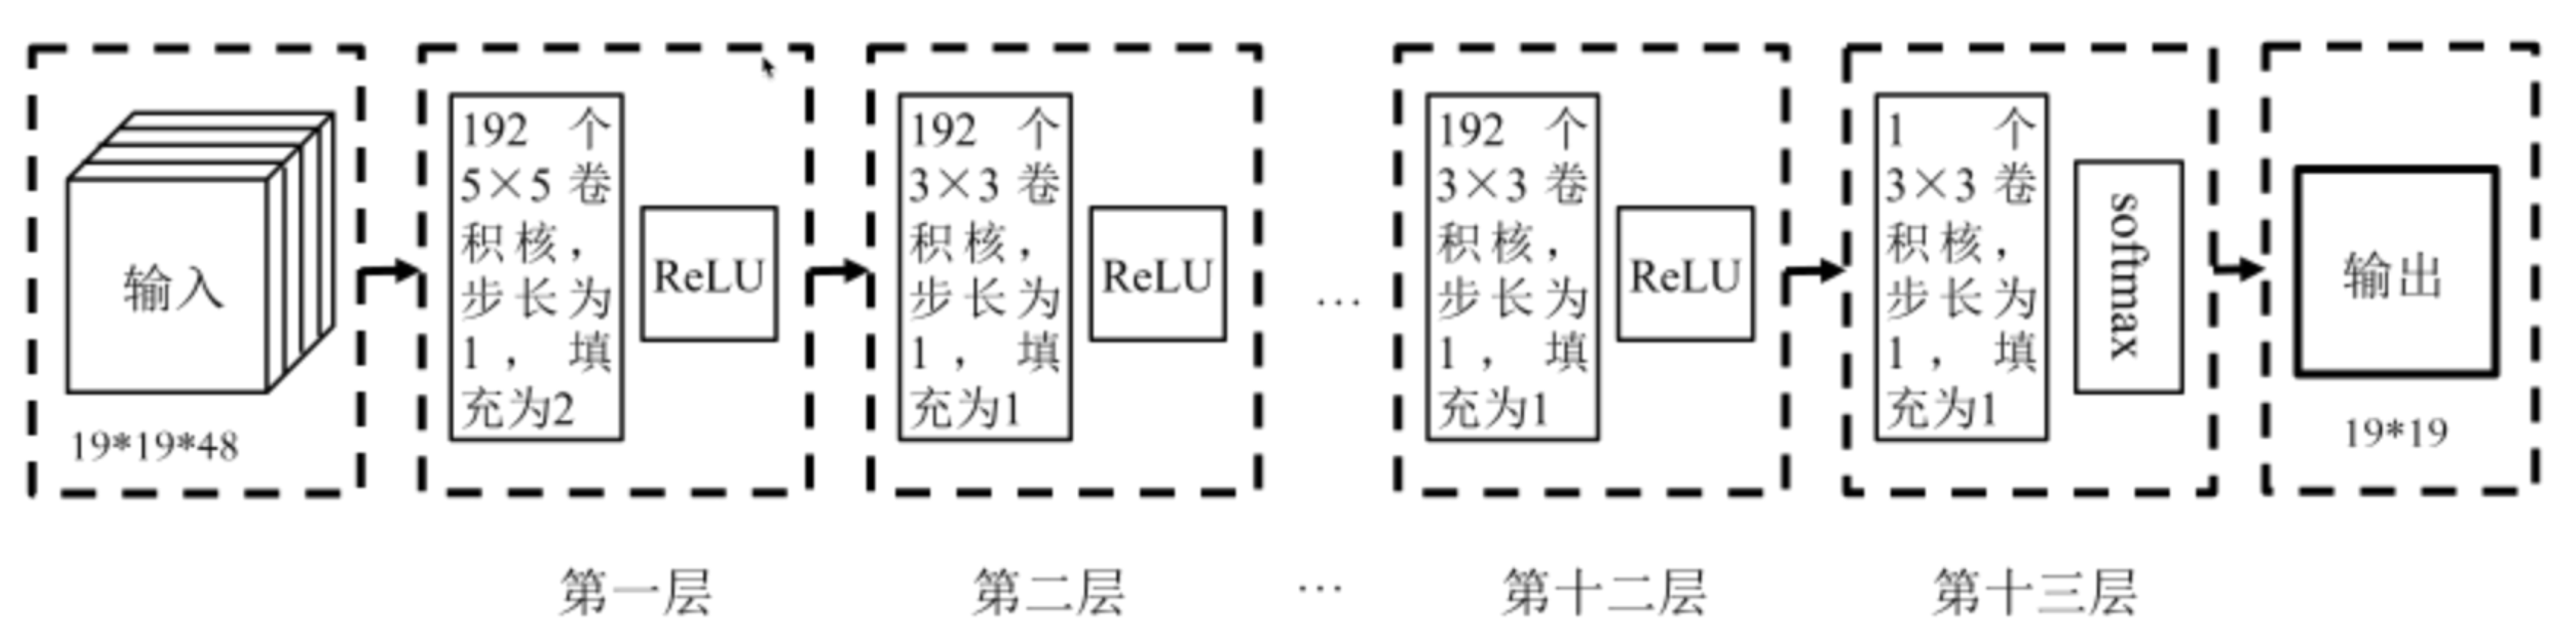
\includegraphics[width=0.95\linewidth]{figs/AlphaGo-policy.png}
    % \caption{4-Queen Example.
    % \vskip 10.1pt%
    \label{fig:AlphaGo-policy}
\end{figurehere}

\textbf{损失函数:}交叉熵,因为一次一个落子所以没有求和。
$L(w) = -t_alog(p_a)$。$t_a=1$:当前棋局棋手落子在 a ,否则为0;$p_a$ :策略网络在 a 处落子概率

\textbf{估值网络\ }

\begin{figurehere}
    \centering    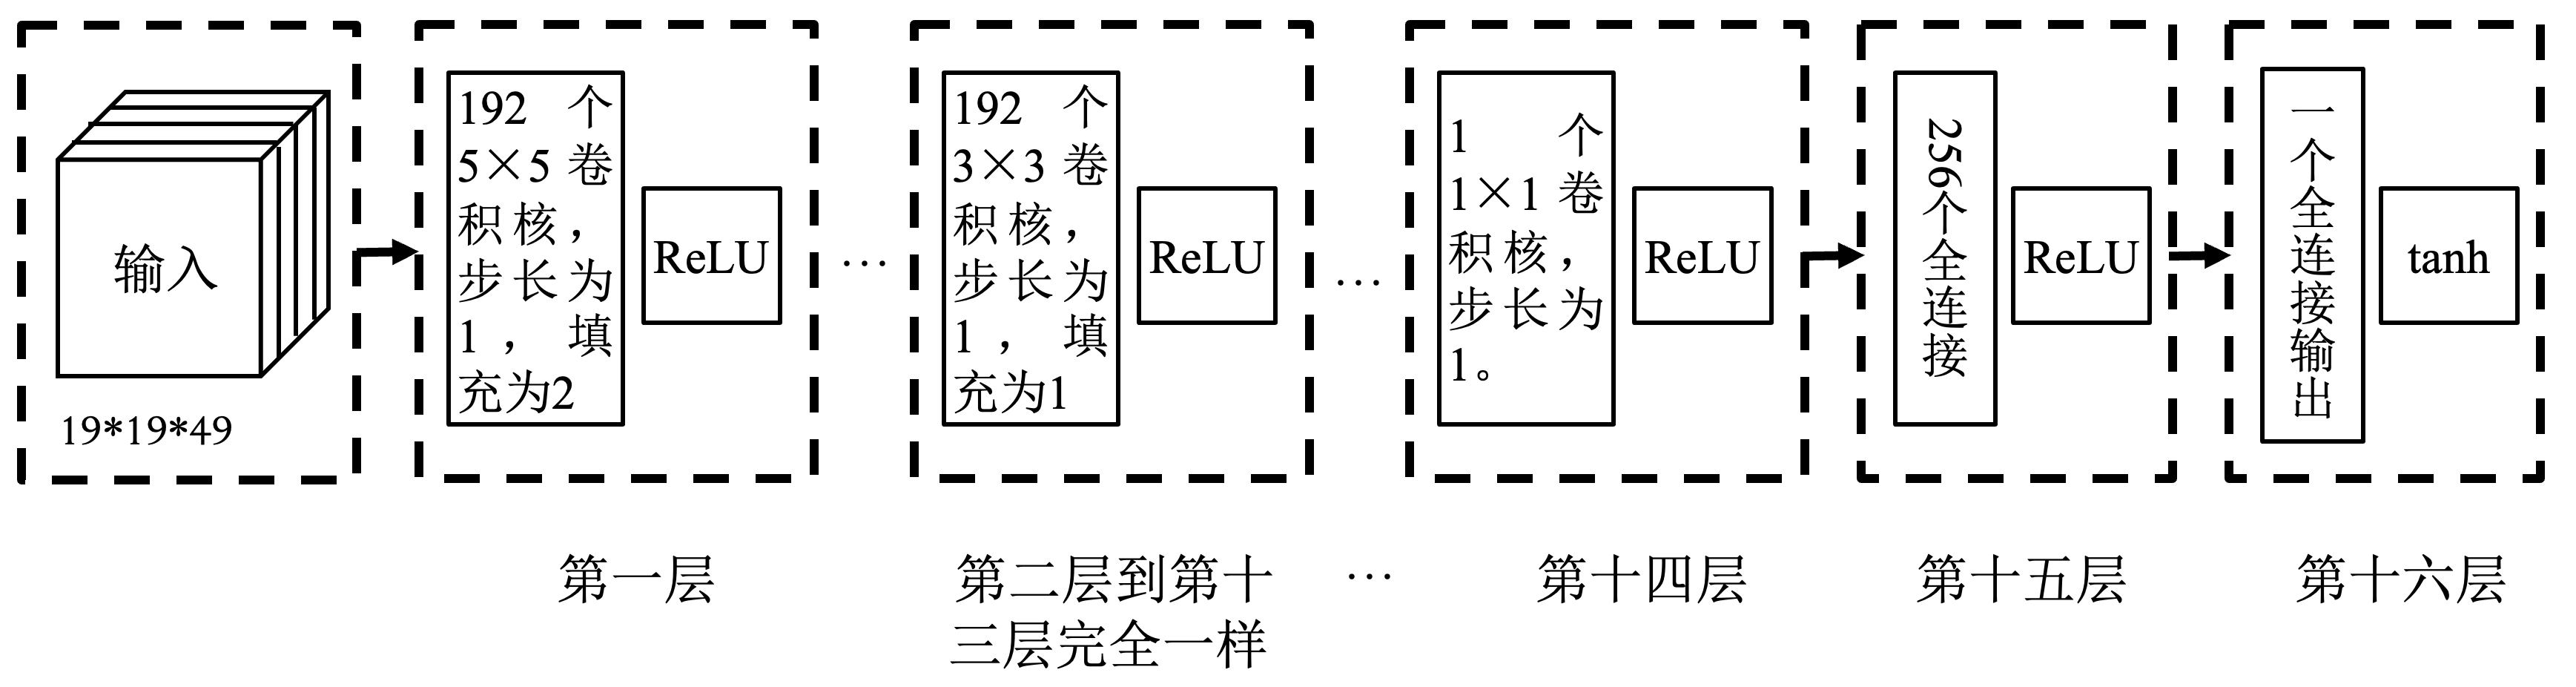
\includegraphics[width=0.95\linewidth]{figs/AlphaGo-value.png}
    % \caption{4-Queen Example.
    \vskip -7pt%
    \label{fig:AlphaGo-value}
\end{figurehere}

训练样本:16万人类棋手数据

等效为一个回归问题:获胜收益为1,失败为-1

损失函数:$L(w)=(R-V(s))^2$,$R$ 是棋局胜负$\{1,-1\}$, $V(s)$ 是估值网络的输出,即预测的收益

\textbf{与蒙特卡洛树搜索融合\ }

MCTS的选择原则:利用;探索

AlphaGo增加了第三个原则:经验(落子概率高)

\textbf{节点 s 第 i 次模拟的收益:}

$v_i(s) = \lambda value(s) + (1-\lambda)rollout(s)$

其中 $value(s)$ 是估值网络输出,$rollout(s)$ 是一次模拟结果(结合快速网络的导向)

\textbf{平均收益:}$Q(s_a) = \frac{\sum_{i=1}^nv_i(s_a)}{n}$
其中 $s_a$ 是在a处落子后的棋局

\textbf{探索项\ } $u(s_a) = c\cdot p(s_a)\frac{\sqrt{N(s)}}{N(s_a)+1}$,
$N(\cdot)$ 是模拟次数,$p(s_a)$ 是策略网络在a处下棋概率,c是加权系数

\textbf{选择过程\ } 用$Q(s_a)+u(s_a)$ 代替信心上限 $I_j$,优先选择该值大的节点;遇到叶子节点结束并选中

\textbf{生成过程\ } 生成 $s_l$ 的所有子节点(概率最大的若干个);\textbf{规定最大节点深度}

\textbf{模拟过程\ } 模拟 $s_l$ 并计算 $v_i(s)$;采用推演(快速)策略网络,并\textbf{规定总模拟次数}

\textbf{回传过程\ } v和-v交替回传到祖先节点

\textbf{节点记录的信息\ } 总收益;行棋到该点的概率;被选择的次数

\textbf{如何确定走步\ } 根节点中被选择次数最多的节点作为最终的走步(而不是看收益/胜率),思想大概是选择“较好且更可信的”

\subsection{围棋中的深度强化学习方法}
\textbf{强化学习\ } 做什么才能让收益最大;学习者不被告知如何做,必须尝试发现哪些动作会产生最大收益

\textbf{两个特征\ } 试错、延迟收益 

\textbf{深度强化学习\ } 用神经网络实现的强化学习

\textbf{关键问题\ } 如何获得指示信号

\textbf{手段\ } 深度强化学习转化为神经网络训练问题;不同转换方法构成了不同的深度学习方法;关键是\textbf{样本的获取}和\textbf{损失函数的定义}

\textbf{围棋中的深度强化学习\ } 自我博弈

\textbf{三种实现方法\ } 策略梯度、价值评估、演员-评价

\subsubsection{基于策略梯度的强化学习}

\textbf{数据:}通过自我博弈产生 $(s,a,p_a,t_a)$

\quad 棋局、行棋点、胜率、最终胜负 $\{1,-1\}$

\textbf{损失函数\ } $L(w)=-t_a log(p_a)$

注:假设获胜者的行为都是正确的,负者的行为都是不正确的;假设负时对权重的修改量的大小与获胜时一样,方向相反(因此$t_a$可以取-1)

\begin{figurehere}
    \centering    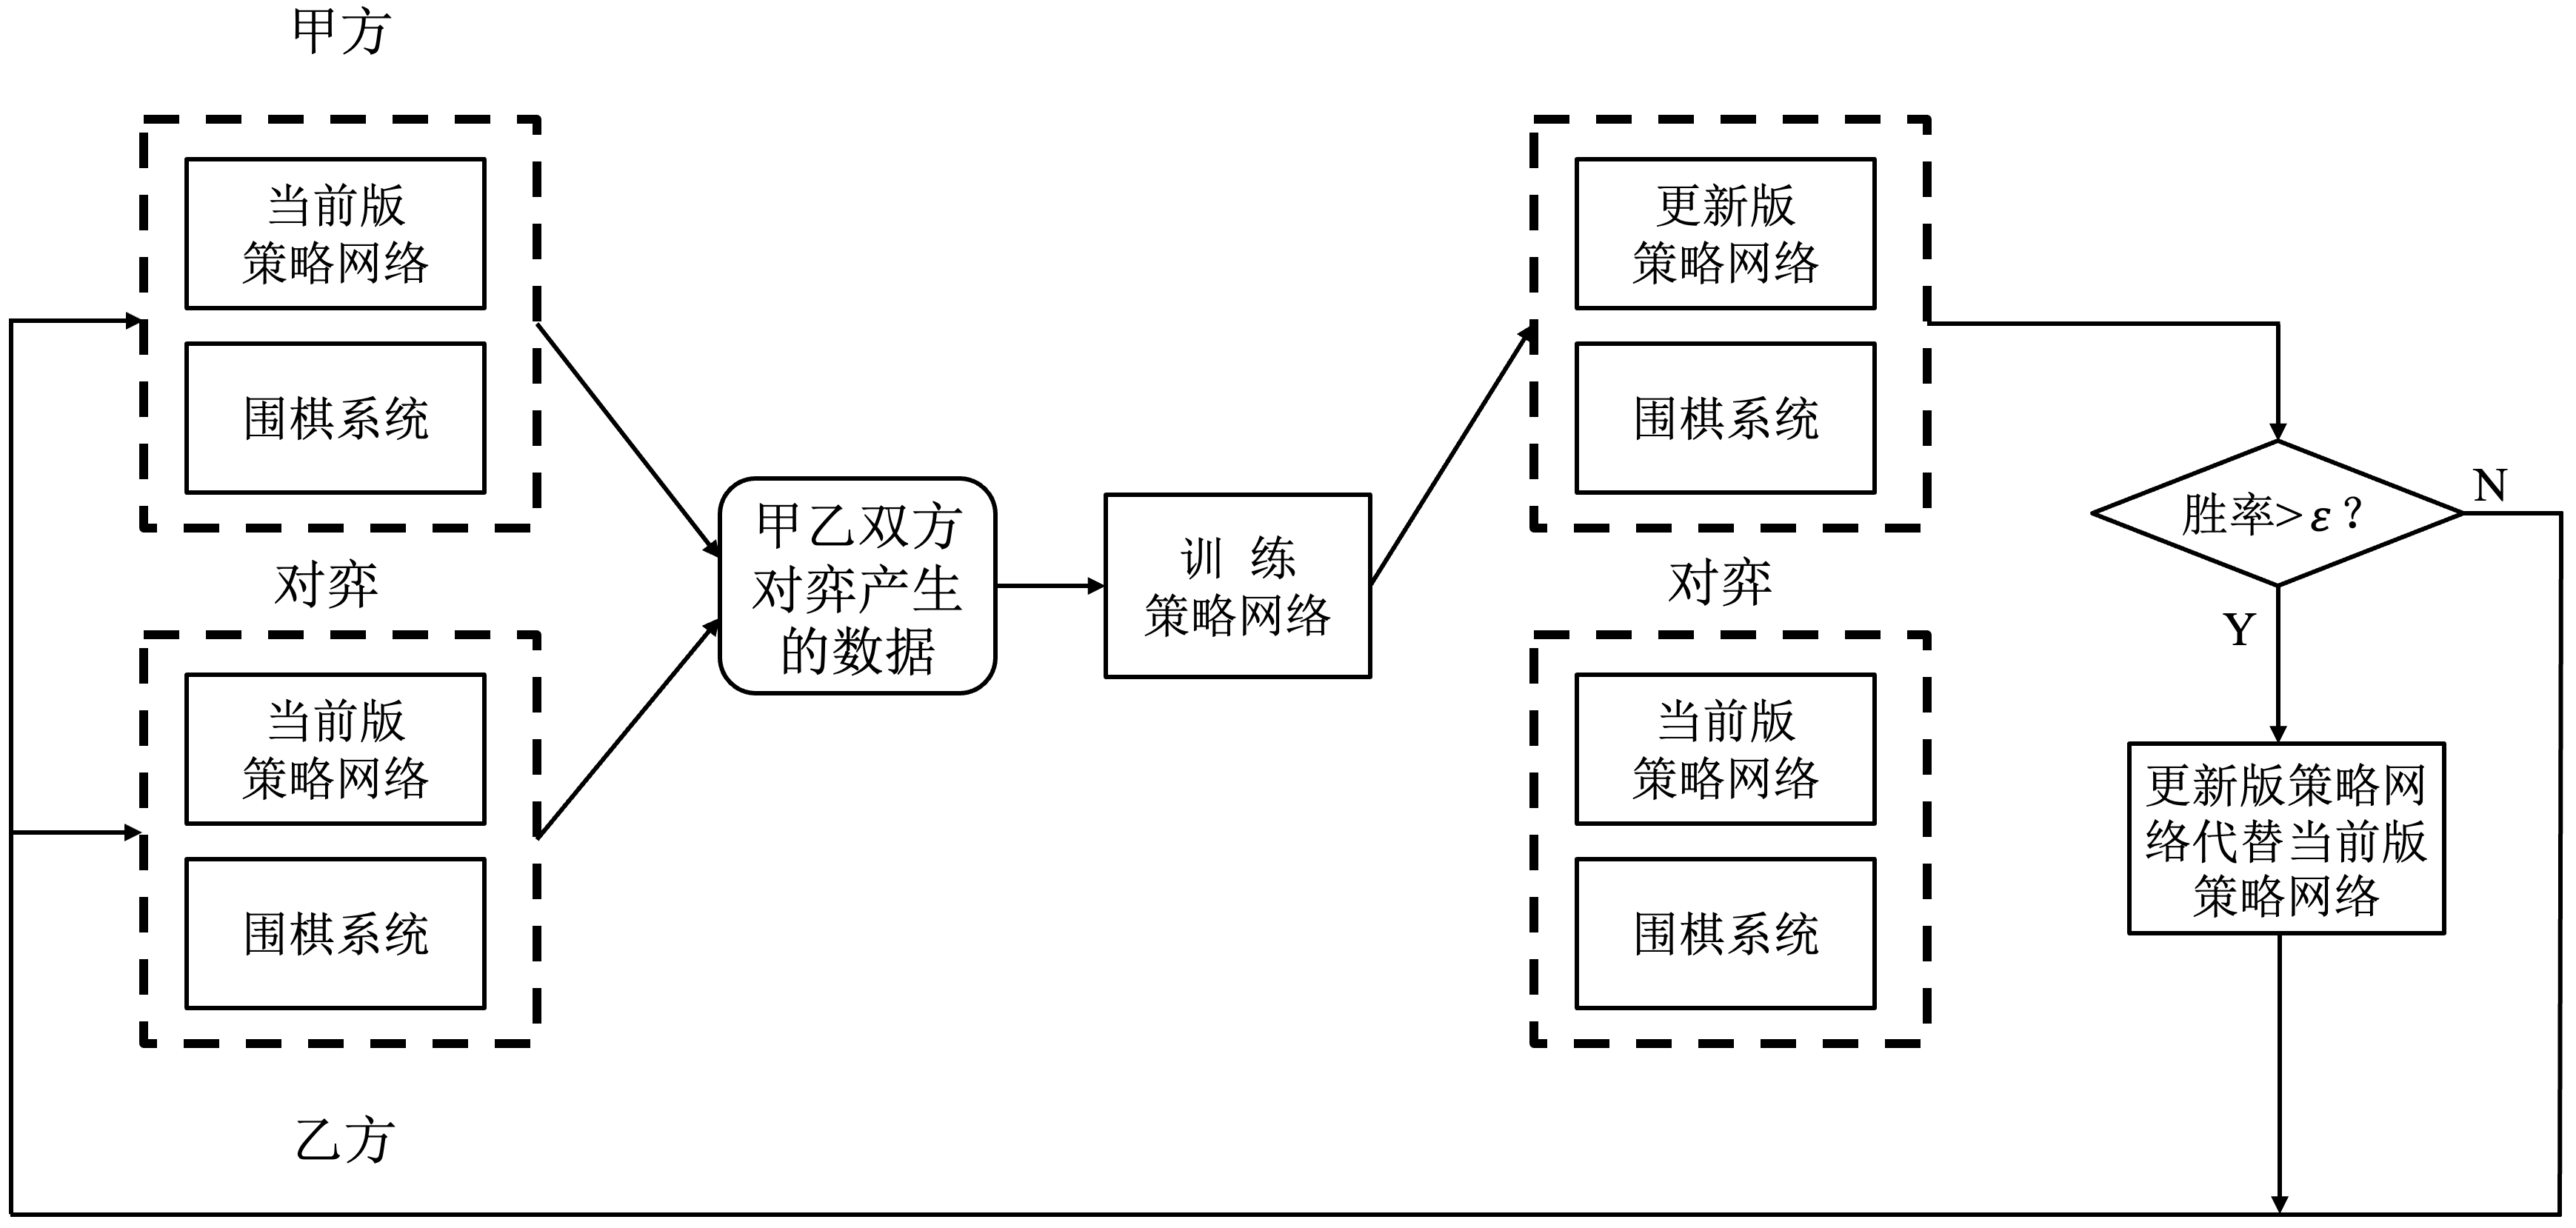
\includegraphics[width=0.95\linewidth]{figs/RL.png}
    % \caption{4-Queen Example.
    % \vskip 10.1pt%
    \label{fig:AlphaGo-RL}
\end{figurehere}

\textbf{注意\ } 强化学习中每个样本只使用一次;基于策略梯度的强化学习学的是每个可落子点的\textbf{获胜概率}(而监督学习策略网络学的是某可落子点行棋概率)

\subsubsection{基于价值评估的强化学习}

\textbf{价值评估网络\ } 评估每一个行棋点的收益

输入:当前棋局和行棋点

输出:$[-1,1]$ 之间的估值

\textbf{数据\ } 自我博弈产生 $(s,a,V(s,a),R)$:当前棋局,行棋点,s下a落子的网络输出,最终胜负\{1,-1\}

\textbf{损失函数\ } $L(w) = (R-V(s,a))^2$

\subsubsection{基于演员-评价方法的强化学习}

同时训练策略网络(棋手)和价值网络(评价)

主要关注关键走步(锦上添花/雪中送炭)

\textbf{收益增量:}评价每一步棋的好坏 $A=Q(s,a)-V(s)$

$V(s)$ 是棋局s的预期收益 [-1,1] (当前网络输出)

$Q(s,a)$ 当前局势s下 在a处行棋的收益 [-1,1]

$A\in [-2,2]$ 反应了一步棋对局势的改变量

\textbf{收益增量计算\ } $A=R-V(s)$,R是胜(1)负(-1)

\textbf{损失函数\ }

评价部分:$L_1(w)=(R-V(s))^2$

演员部分:$L_2(w)=-Alog(p_a)$

综合损失函数:$L(w)=L_1(w)+\lambda L_2(w)$

\begin{figurehere}
    \centering    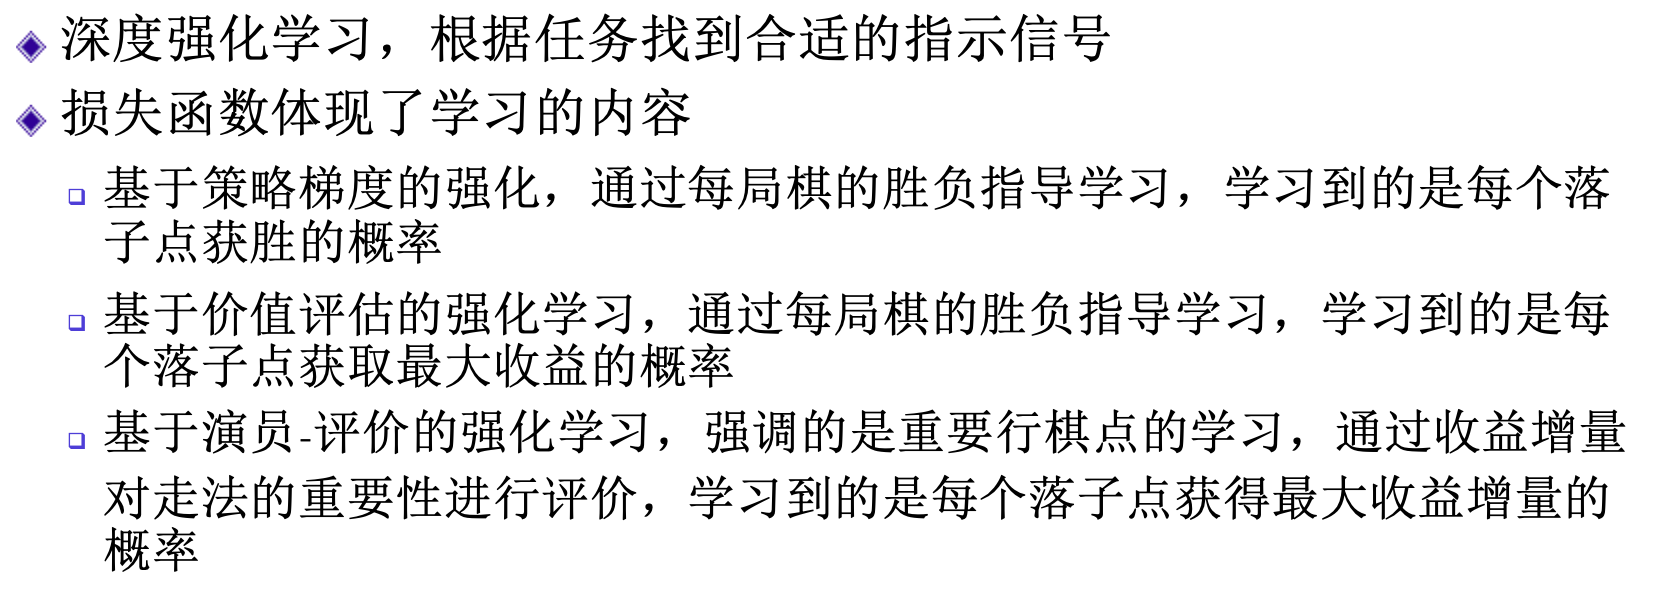
\includegraphics[width=0.95\linewidth]{figs/DRL.png}
    % \caption{4-Queen Example.
    % \vskip 10.1pt%
    \label{fig:AlphaGo-DRL}
\end{figurehere}

\subsection{AlphaGo Zero 原理}
实现从零学习,不使用人类棋手(16万盘)+人工特征(48通道)数据输入,\textbf{利用强化学习}从零学习

思路:强化学习+蒙特卡洛

% 58:00

\textbf{网络结构\ } 合并策略网络估值网络为“双输出”网络 

输入:17个通道,其中16个记录到目前为止的8个通道(黑白各一个通道);当前行棋方(黑1白0)

策略网络输出:19*19+1,外加一个“放弃”行为

估值网络输出:当前棋局的估值 $\in [-1,1]$

\begin{figurehere}
    \centering    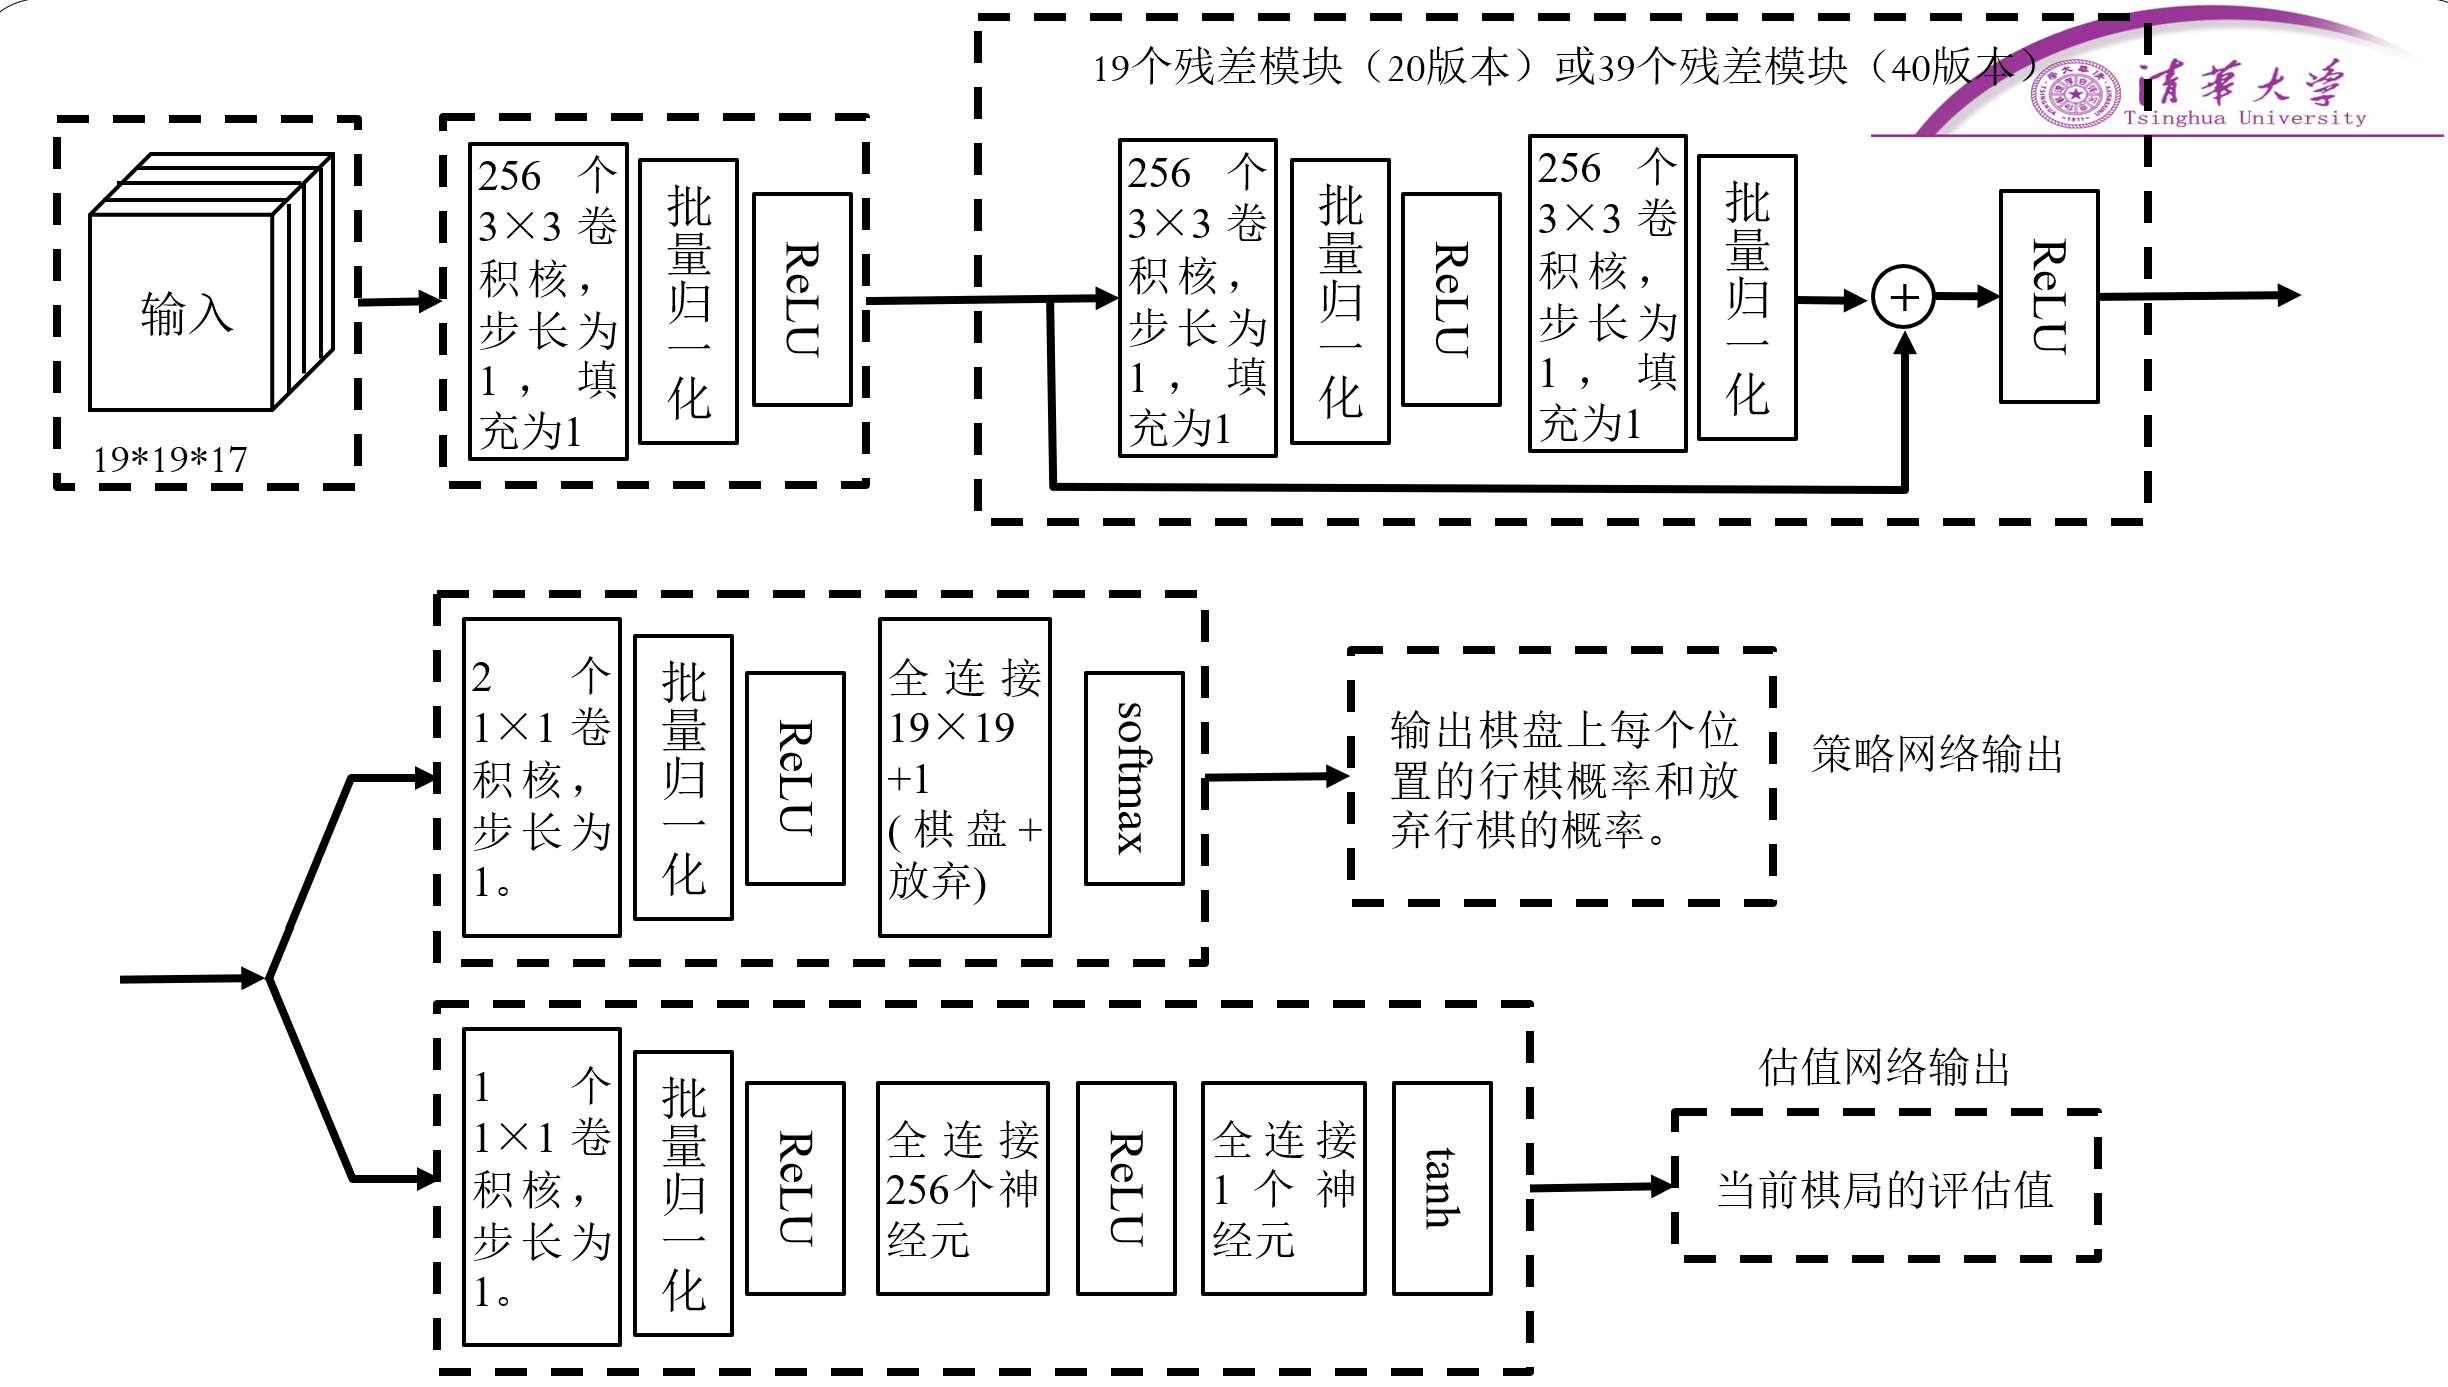
\includegraphics[width=0.99\linewidth]{figs/AlphaGo-Zero.png}
    % \caption{4-Queen Example.
    % \vskip 10.1pt%
    \label{fig:AlphaGo-Zero}
\end{figurehere}

\textbf{批量归一化\ } 每个批量完成之后,对卷积层的输出做一次均值为 0 方差为 1 的归一化,防止数据漂移

\textbf{AlphaGo Zero 中的 MCTS\ }

为什么需要模拟?对比AlphaGo的MCTS

$v_i(s)=value(s)$ 仅使用估值网络,去掉模拟

\textbf{选择}依据仍然是 $Q(s_a)+u(s_a)$

\textbf{生成}所有的子节点,与AlphaGo一样

\textbf{模拟}过程用估值网络输出取代

\textbf{回传}也是一次正一次负

\textbf{AlphaGo-Zero 结合蒙特卡洛\ }

\textbf{损失函数:}

估值网络:$L_1 = (z-v)^2$,其中 z 是胜1负-1,v是估值网络输出

策略网络:$L_2 = -\sum_{i=1}^{362} \pi_i log(p_i)$,其中 $\pi_i$ 是MCTS给出的每个落子点(含放弃)的概率;$p_i$ 是策略网络输出的每个落子点(含放弃)的概率

总损失函数:$L=L_1+L_2+||\theta||^2_2$

\textbf{如何获得$\pi_i$\ } 把节点的\textbf{选中次数}转换为概率

\textbf{引入多样性\ } 对策略网络的输出人为引入噪声

狄利克雷分布:通过控制参数产生一些符合一定条件的概率分布

控制参数:n:概率分布向量长度;$\alpha$:分布浓度
% \begin{itemize}
%     \item 
%     \item 
% \end{itemize}

落子概率=$\lambda p_a+(1-\lambda)p_d$

$p_a$ 策略网络输出,$p_d$ 狄利克雷分布采样

目的:扩大探索范围

\textbf{AlphaGo-Zero 的强化学习过程\ } 和3.6.1的图几乎一样,其中“围棋系统”改为“蒙特卡洛树搜索”


\section{统计学习方法}
% 统计学习就是计算机系统通过运用数据及统计方法提高系统性能的机器学习(是有理论指导的)

% 统计学习从数据出发,提取数据的特征,抽象出数据的模型,发现数据中的知识,又回到对数据的分析与预测中。

% 统计学习的目标就是考虑学习什么样的模型和如何学习,以使模型能对数据进行准确的预测和分析

\textbf{三要素\ } 模型、策略、算法
% \begin{itemize}
%     \item 模型:学习什么样的模型(条件概率分布、决策函数)
%     \item 策略:模型选择的准则(经验风险最小化、结构风险最小化)
%     \item 算法:模型学习的算法(一般归结为一个最优化问题)
% \end{itemize}

\textbf{统计机器学习分类\ } 监督、非监督、半监督、弱监督学习(强化学习属于弱监督)

\subsection{支持向量机SVM}
% 二分类(可组合解决多分类问题)

特征空间上的间隔最大化线性分类器

% 通过核函数可以实现非线性分类

% 根据模型复杂度的分类
% \begin{itemize}
%     \item 线性可分支持向量机
%     \item 线性支持向量机
%     \item 非线性支持向量机
% \end{itemize}

\subsubsection{线性可分支持向量机}

\textbf{最优分界面\ } $w\cdot x + b = 0$

\textbf{定义4.1:}给定线性可分训练集:
其中:
$T=\{(x_1,y_1),\dots,(x_N,y_N)\},x_i\in X=R^n,y_i\in Y=\{+1,-1\},i=1,2,\dots,N$
这里 $x_i$ 为第 $i$ 个特征向量,$y_i$ 为 $x_i$ 的类标记,+1表示正类,-1表示负类。
通过间隔最大化得到分类超平面:$w^*\cdot x + b^* = 0$,
相应的决策函数:$f(x)=sign(w^*\cdot x + b^*)$
称为线性可分支持向量机

\begin{figurehere}
    \centering    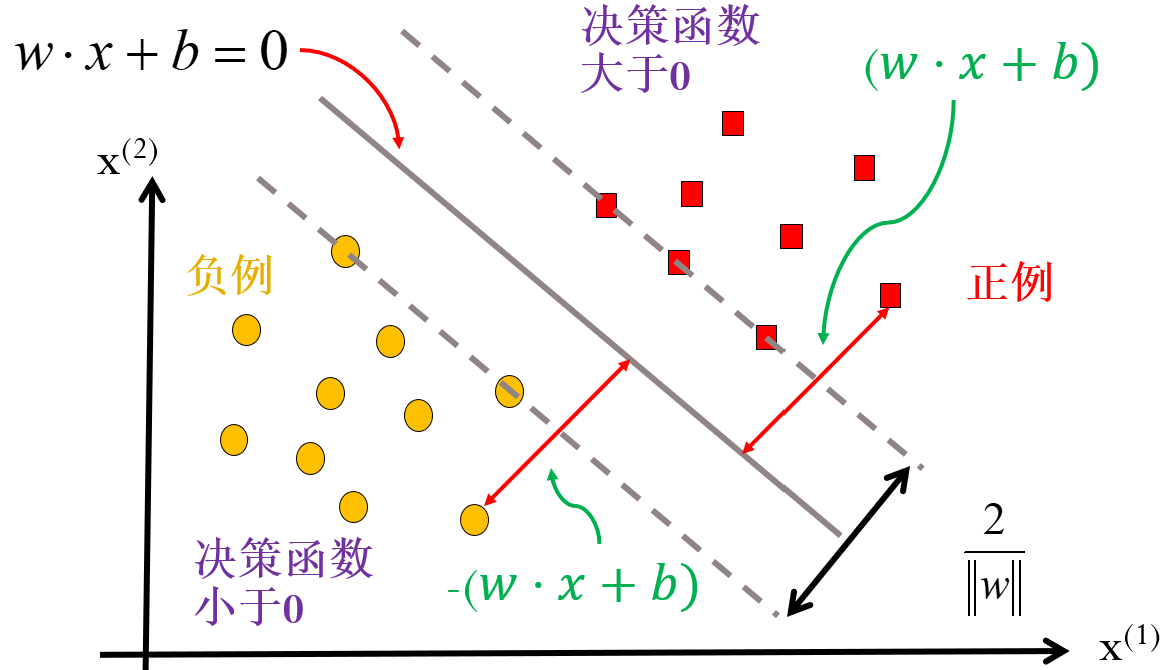
\includegraphics[width=0.99\linewidth]{figs/linerSVM.png}
    % \caption{4-Queen Example.
    \vskip -7pt%
    \label{fig:linerSVM}
\end{figurehere}

\textbf{函数间隔\ } 设训练集 T 和超平面 (w,b),定义超平面 (w,b) 关于样本点 ($x_i,y_i$) 的函数间隔为

$\hat{\gamma}_i = y_i(w\cdot x_i+b)\ge 0$

定义超平面关于训练集 T 的函数间隔为 $\hat{\gamma} = \underset{i}{min} \hat{\gamma}_i$ 

% 注:超平面方程可以以参数k任意缩放

\textbf{几何间隔\ }

$\gamma_i = y_i(\frac{w}{||w||}\cdot x_i+\frac{b}{||w||})$, 
$\gamma = \underset{i}{min} \gamma_i$ 

其中 $||w||$ 为 w 的 $L_2$ 范数(归一化)

\textbf{间隔最大化\ }
$
\underset{w,b}{max}\  \gamma
$

$
s.t.\ \gamma_i = y_i(\frac{w}{||w||}\cdot x_i+\frac{b}{||w||}) \ge \eta, i=1,2,\dots,N
$

函数间隔表示:
$
\underset{w,b}{max}\ \frac{\hat{\gamma}}{||w||}
$

$
s.t.\ y_i(w\cdot x_i+b)\ge \hat{\gamma},i=1,2,\dots,N
$

可取 $\hat{\gamma} = 1$,转化为如下凸二次规划问题:

$
\underset{w,b}{min} \frac{1}{2}||w||^2
$, 
$
s.t.\ y_i(w\cdot x_i+b)\ge 1, i=1,2,\dots,N
$

\textbf{学习的对偶算法\ } 原始问题如上,改写如下:

$
\underset{w,b}{min} \frac{1}{2}||w||^2
$,
$
s.t.\ 1 - y_i(w\cdot x_i+b)\le 0, i=1,2,\dots,N
$

拉格朗日函数:( $\alpha_i \ge 0$ 是拉格朗日乘子)

$L(w,b,\alpha) = \frac 1 2 ||w||^2 + \sum_{i=1}^N \alpha_i[1-y_i(w\cdot x_i + b)]$,

因此 $\underset{\alpha}{max}(L(w,b,\alpha)) = \begin{cases}
    \frac{1}{2} ||w||^2, \mbox{当满足约束}\\
    \infty, \mbox{其他}
\end{cases}$

因此 $\underset{w,b}{min} \underset{\alpha}{max} (L(w,b,\alpha))$
 与原始问题等价

\textbf{对偶问题\ } 

$\underset{w,b}{min} \underset{\alpha}{max}(L(w,b,\alpha)) \Rightarrow \underset{\alpha}{max}\underset{w,b}{min}(L(w,b,\alpha))$

$\underset{w,b}{min}(L(w,b,\alpha))\le L(w,b,\alpha)\le \underset{\alpha}{max}(L(w,b,\alpha))$

即 $\underset{w,b}{min} \underset{\alpha}{max}(L(w,b,\alpha)) \le \underset{\alpha}{max}\underset{w,b}{min}(L(w,b,\alpha))$

当满足下述KKT条件时上述等号成立:

$\nabla_{w,b} L(w,b,\alpha) = 0$

$\alpha_i[1-y_i(w\cdot x_i+b)]=0$

$1-y_i(w\cdot x_i+b)\le 0$

$\alpha_i \ge 0, i=1,2,\dots,N$


对偶问题的求解:对w,b求偏导,令其为0代入

$
\underset{\alpha}{max} (-\frac{1}{2}\sum_{i=1}^N \sum_{j=1}^N \alpha_i \alpha_j y_iy_j (x_i\cdot x_j) + \sum_{i=1}^N \alpha_i
)$

$
s.t. \sum_{i=1}^N \alpha_iy_i=0, \alpha_i\ge 0,i=1,2,\dots,N
$

等价于\textbf{(重要结论,线性可分支持向量机算法)}

$
\underset{\alpha}{min} (\frac{1}{2}\sum_{i=1}^N \sum_{j=1}^N \alpha_i \alpha_j y_iy_j (x_i\cdot x_j) - \sum_{i=1}^N \alpha_i
)$

$
s.t. \sum_{i=1}^N \alpha_iy_i=0, \alpha_i\ge 0,i=1,2,\dots,N
$

再利用KKT条件中的前两条:

$
w^* = \sum_{i=1}^N \alpha^*_iy_ix_i
$

$
b^* = y_j - \sum_{i=1}^N \alpha_i^* y_i (x_i \cdot x_j) (\mbox{选择一个}\alpha^*_j>0\mbox{的计算})
$

其中 $\alpha_i^*>0$ 的就是支持向量(产生等式约束)

注:若求出 $\alpha_i<0$,则说明最小值在边界

\subsubsection{线性支持向量机}
不一定线性可分,线性可分的支持向量函数距离=1

如果某些点线性不可分,则引入松弛变量:

$y_i(w\cdot x_i+b)\ge 1-\xi_i, i=1,2,\dots,N,\xi_i\ge 0$

优化目标:$\underset{w,b,\xi}{min} (\frac{1}{2} ||w||^2 + C\sum_{i=1}^N \xi_i)$

\textbf{线性支持向量机的对偶问题:}

$
\underset{\alpha}{min} (\frac{1}{2}\sum_{i=1}^N \sum_{j=1}^N \alpha_i \alpha_j y_iy_j (x_i\cdot x_j) - \sum_{i=1}^N \alpha_i
)$

$
s.t. \sum_{i=1}^N \alpha_iy_i=0, 0\le \alpha_i\le C,i=1,2,\dots,N
$

求最优解 $\alpha^*$,计算$w^*$,选一个满足 $0\le \alpha_j^* \le C$ 的 $\alpha_j$ 计算 $b^*$

\textbf{一些结论\ }

$\alpha_i^*>0$ 对应的样本 $x_i$ 称为(软间隔)支持向量;若 $\alpha_i^* < C$ 则 $\xi_i = 0$, $x_i$ 在间隔边界上;若 $\alpha_i^*=C$,$0\le \xi_i \le 1$ 则分类正确,$x_i$ 在间隔边界和分离超平面之间;若 $\alpha_i^*=C,\xi=1$,则 $x_i$ 在超平面上;若 $\alpha_i^*=C,\xi_i>1$,则$x_i$ 在误分一侧

\subsubsection{非线性支持向量机}
基本思想:变换 $\Phi(x)$ →线性支持向量机

\textbf{核函数\ } 
设X是输入空间,H是特征空间,如果存在
$\Phi(x): X \to H$
使得对所有 $x,z\in X$,函数 $K(x,z)$满足:
$K(x,z)=\Phi(x)\cdot \Phi(z)$,("$\cdot$"表示内积)
则称 $K(x,z)$为核函数,$\Phi(x)$为映射函数

注:核函数对应的映射函数可能不唯一

\textbf{非线性支持向量机算法(支持向量机一般形式)\ }

$
\underset{\alpha}{min} (\frac{1}{2}\sum_{i=1}^N \sum_{j=1}^N \alpha_i \alpha_j y_iy_j K(x_i, x_j) - \sum_{i=1}^N \alpha_i
)$

$
s.t. \sum_{i=1}^N \alpha_iy_i=0, 0\le \alpha_i\le C,i=1,2,\dots,N
$

选择一个 $0\le \alpha_j^* \le C$ 的计算 

$b^* = y_j - \sum_{i=1}^N \alpha_i^* y_i K(x_i,x_j)$

$w^* = \sum_{i=1}^N \alpha_i^* y_i \Phi (x_i)$(实际无法求出)

超平面:$w^*\cdot \Phi(x) + b^* = 0$,代入 $w^*$

$\sum_{i=1}^N \alpha_i^* y_i K(x_i,x) + b^*=0$

决策函数:$f(x)=sign(\sum_{i=1}^N \alpha_i^* y_i K(x_i,x) + b^)$

\textbf{常用核函数\ }
\begin{itemize}
    \item 多项式核函数:$K(x,z)=(x\cdot z+1)^p$
    \item 高斯核函数:$K(x,z)=exp(-\frac{||x-z||^2}{2\sigma^2})$
\end{itemize}

对于高斯核函数:$\sigma$ 较大时欠拟合,较小过拟合


\textbf{序列最小最优化算法SMO\ } 速解凸二次规划
% 可以快速求解支持向量机使用的凸二次规划问题

% 支持向量机相比深度学习具有更好的理论保障

\subsubsection{SVM用于求解多分类问题}
\begin{itemize}
    \item 一对多:某一类当成正类,其他为负类;将样本分给具有最大分类值的类(去掉符号函数)
    \item 一对一:任意两类构造一个SVM,投票法
    \\(效果最好,但支持向量机个数最多)
    \item 层次法:所有类先分两类,再细分
\end{itemize}

通用问题:多样本不平衡问题

\subsubsection{SVM应用举例:文本分类}

\textbf{文本向量空间模型\ } $(w_{1,j},w_{2,j},\dots,w_{n,j})^T$,其中 $w_{i,j}$ 表示词i在文档j中的权重

词频:$tf_{ij}$ ——词i在文档j中的权重

逆文档频率:$idf_i=log(1/df_i)$,其中 $df_i=$ 含有词i的文档数/文档总数 N

TF-IDF权重:$w_{ij}=tf_{ij}\times idf_i$ 以及其他变形

\subsection{决策树}
% 决策树模型是一种描述对实例进行分类的树形结构,由节点和有向边组成。节点有两种类型:内部节点和叶节点。
内部节点表示一个特征或属性,叶节点表示一个类。

% 但是会有组合爆炸问题,不可能穷举

\textbf{决策树学习\ } 

给定训练集 $D=\{(x_1,y_1),(x_2,y_2),\dots,(x_N,y_N)\}$,其中 $x_i=(x_i^{(1)},\dots,x_i^{(n)})$ 为输入实例,n为特征个数,$y_i\in \{1,2,\dots,K\}$ 为类标记,$i=1,2,\dots,N$,N是样本容量
% \begin{figurehere}
%     \centering    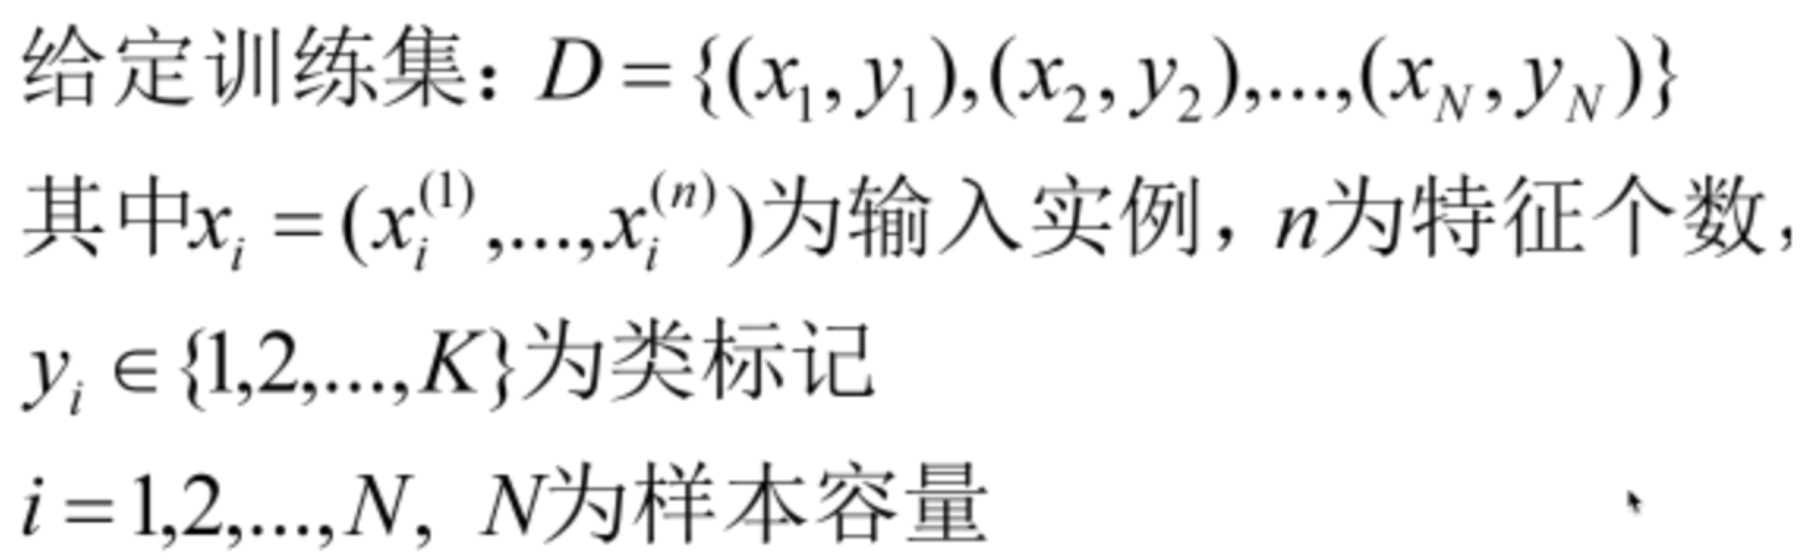
\includegraphics[width=0.99\linewidth]{figs/DecisionTree.png}
%     % \caption{4-Queen Example.
%     % \vskip 10.1pt%
%     \label{fig:DecisionTree}
% \end{figurehere}

从训练集中归纳一组分类规则,得到一个与训练集矛盾较小的决策树;常用启发式方法得到一个\textbf{近似解};决策树学习包括特征选择、决策树生成与剪枝 

\textbf{特征选择\ } 决策树中一般按照信息增益选择特征

\textbf{信息增益:} 某个特征A对数据集D进行分类的不确定性减少的程度

\textbf{随机变量X的熵:}$H(X)=-\sum_{i=1}^n p_ilogp_i, p_i=P(X=x_i)$,也记作 $H(p)$。由数据集D估计得概率记作$H(D)$

条件熵:$H(Y|X)=\sum_{i=1}^{n} p_i H(Y|X=x_i)$

\textbf{信息增益\ } 特征A对数据集D的信息增益定义为:

$g(D,A)=H(D)-H(D|A)$

即特征A对数据集D的不确定性的减少程度

设数据集 D 由K个类别 $C_k$,特征 A 有 n 个不同的取值 $\{a_i,\dots a_n \}$,A的不同取值将D划分为n个子集 $D_1\dots D_n$,$D_i$ 中属于类 $C_k$ 的样本的集合为 $D_{ik}$,$|\cdot|$ 表示样本的个数。

信息增益计算公式:
$
g(D,A) = H(D) - D(D|A)
$

$
H(D) = -\sum_{k=1}^K \frac{|C_k|}{|D|} log_2 \frac{|C_k|}{|D|}
$

$
H(D|A) = \sum_{i=1}^n \frac{|D_i|}{|D|} 
$

$
H(D_i)=-\sum_{i=1}^n \frac{|D_i|}{|D|}\sum_{k=1}^K \frac{|D_{ik}|}{|D_i|} log_2\frac{|D_{ik}|}{|D_i|}
$

\subsubsection{ID3算法}

输入:训练集D,特征集A,阈值 $\epsilon > 0$

输出:决策树T

1. 若D中所有的实例属于同一类 $C_k$,则T为单节点树,$C_k$ 作为该节点类标记,返回T

2. 若 A 为空,则 T 为单节点树,将 D 中实例数最大的类 $C_k$ 作为该节点的类标记,返回T

3. 否则计算 A 中各个特征对 D 的信息增益,选择信息增益最大的特征 $A_g$

4. 如果 $A_g$ 的信息增益小于阈值 $\epsilon$,则置 T 为单节点树,将D中的实例树最大的类 $C_k$ 作为该节点的类标记,返回 T

5. 否则对 $A_g$ 中的每一个可能值 $a_i$,依 $A_g=a_i$ 将 D 分割为若干子集 $D_i$,作为 D 的子节点

6. 对于 D 的每一个子节点 $D_i$,如果 $D_i$ 为空,则将 $D$ 中的实例最大的类作为标记,构建子节点

7. 否则以 $D_i$ 为训练集,以 $A-\{A_g\}$ 为特征集,递归地调用1-6步,得到子树 $T_i$,返回 $T_i$

\textbf{例题\ } 先算数据集熵,然后算各特征信息增益

\textbf{ID3的问题\ } 信息增益倾向于选择分支较多的属性

\subsubsection{C4.5算法}

\textbf{信息增益比\ } 类比相对误差

$
g_R(D,A) = \frac{g(D,A)}{H_A(D)}
$,
$
H_A(D) = -\sum_{k=1}^n \frac{
|D_k|}{|D|} log_2 \frac{|D_k|}{|D|}
$

其中 A 是属性(特征),A取值不同将D划分为不同子集(按照特征分,与最终分类无关)

$H_A(D)$ 在分类很多且均匀分布的时候会比较大

\textbf{C4.5的生成算法\ } 除了根据信息增益比选择特征之外,C4.5算法与ID3基本一样;此外,C4.5增加了对连续值属性的处理,对于连续值A,找到一个属性值 $a_0$,将 $\le a_0$ 的划分到左子树,$a>a_0$ 的划分到右子树(找信息增益比最大的切分)

注意:连续值属性在子节点可以继续使用

\textbf{信息增益比的问题\ } 倾向于选择分割不均匀的特征

\textbf{解决方式\ } 先选择 n 个信息增益大的特征,再从中选择信息增益比最大的特征

\subsubsection{过拟合问题}
\textbf{问题现象\ } 树规模↑,训练集↑,测试集先↑后↓

\textbf{一种解决方法-后剪枝\ } 先建树,再剪枝

把一个有儿子的节点合并成一个叶子节点,选择类别最大的作为节点标记。当性能不再提高时停止。

当数据量小时:直接利用训练集进行剪枝

\textbf{定义损失函数\ } 树 T 的叶节点个数为 |T|,t是树T的叶子结点,该节点有 $N_t$ 个样本,其中 $k$ 类的样本点有 $N_{tk}$ 个 $(k=1,\dots,K)$,$H_t(T)$ 为叶子结点t上的经验熵,$a\ge 0$ 为参数

$C_a(T) = \sum_{t=1}^{|T|}N_tH_t(T)+a|T|$

其中经验熵 $H_t(T)=-\sum_k \frac{N_{tk}}{N_t}log \frac{N_{tk}}{N_t}$

\textbf{决策树剪枝算法\ }

输入:生成算法产生的整棵树T,参数a

输出:修剪后的子树 $T_a$

1. 计算每个节点的经验熵

2. 递归地从树的叶节点向上回缩,若回缩后的损失函数 $\le$ 回缩前,则剪枝,将父节点变为新的叶节点

3. 返回2,直到不能继续为止,得到损失函数最小的子树 $T_a$

\subsubsection{随机森林}
\textbf{问题\ } 决策树容易过拟合

\textbf{解决方案\ } 使用多个决策树组成随机森林,构成分类器;采用投票机制改善决策树;(有放回的)随机采样(数据/特征)构建单个决策树

多个过拟合之间有消解,所以可以不用剪枝
% $L=|T|+\mbox{误差}$




% \section{预备知识}

% \subsection{集合与映射}

% \textbf{常见数集} $\setN, \setZ, \setQ, \setR, \setC$

% \textbf{幂集} A所有子集构成集合,$\powerset{A}$或$2^A$

% \textbf{映射} $f: A \to B, x \mapsto f(x) \in B$

% \begin{itemize}
%     \item[\emph{单射}] $\forall x_1, x_2 \!\in\! A, x_1 \!\neq\! x_2 \!\impl\! f(x_1) \!\neq\! f(x_2) $
%     \item[\emph{满射}] $f(A) \! = \! B \impl \forall y \!\in\! B, \exists x \!\in\! A, f(x) = y$
%     \item[\emph{双射}] 单射且满射 $\impl$ 可逆
% \end{itemize}

% \textbf{变换} $f: A \to A$,$f$是A上的变换

% \textbf{复合映射} $fg(x) = f(g(x))$

% \textbf{恒等变换} $I_A(x) = x$

% \textbf{映射的逆} $gf \! = \! I_A, fh \! = \! I_B \impl g \! = \! h \!= \! f^{-1}$

% \subsection{二元关系}

% \textbf{二元运算} $f: S \times S \to S$

% \textbf{二元关系} $\forall a \!\in\! A, b \!\in\! B$可判$\!aRb\!$或$\!aR'b\!$

% \textbf{等价关系} $\sim$是等价关系$\iff$满足

% \begin{itemize}
%     \item[\emph{反身}] $\forall a \!\in\! A, a \sim a$
%     \item[\emph{对称}] $\forall a, b \!\in\! A, a \sim b \impl b \sim a$
%     \item[\emph{传递}] $\forall a, b, c \!\in\! A, a \sim b, b \sim c \impl a \sim c $
% \end{itemize}

% \textbf{等价类} $\bar{a} = \{ x | x \in A, x \sim a \}$ \textbf{代表元}$a$

% \textbf{划分} $\{ A_\alpha | \alpha \in I \}$ 是划分$\iff$满足

% \begin{itemize}
%     \item $\bigcup\limits_{\alpha \in I} A_\alpha = A$
%     \item $\forall \alpha, \beta \in I, \alpha \ne \beta, A_\alpha \bigcap A_\beta = \emptyset$
% \end{itemize}

% \begin{theorem}[等价与划分]
%     $a \sim b \iff \exists \alpha \in I, a, b \in A_\alpha$
% \end{theorem}

% \textbf{商集} $A/\sim = \{ \bar{a} | a \in A \}$

% \textbf{偏序} 反身、反对称、传递

% \textbf{全序} 偏序且$\forall x, y \in S, x \leq y$或$y \leq x$

% \subsection{整数与同余}

% \begin{theorem}[Bézout定理]
%     $a, b \in \setZ^*, \exists p, q \in \setZ \st pa + qb = \gcd(a, b) = d$ \quad[辗转相除求p, q]
% \end{theorem}

% \begin{theorem}[gcd \& lcm]
%     $(a, b)[a, b] = ab$
% \end{theorem}

% \textbf{一次同余方程} $ax \!\equiv\! b \pmod{m} \iff (a, m) \!\mid\! b$\\
% 通解$x \!\equiv\! pb_1 \pmod{m_1}\ [a \!\! = \!\! a_1(a, m), b \!\! = \!\! b_1(a, m), \\ m = m_1(a, m), pa_1 +qm_1 = 1]$

% \textbf{一次同余方程组} $\begin{cases}
%         x \equiv b_1 \pmod{m_1} \\
%         x \equiv b_k \pmod{m_k}
%     \end{cases}$\\
% 通解$x \equiv \sum_{i=1}^k b_i c_i M_i \pmod{M}$\\
% $M \! = \! \prod\limits_{i=1}^k m_i, M_i \! = \! \frac{M}{m_i}, M_i c_i \equiv 1 \pmod{m_i}$

% \section{群论}

% \subsection{概念与例子}

% \textbf{群} $(G, \cdot)$ 封结幺逆(交)

% \begin{theorem}[幺元性质]
%     $e_L = e_R = e$
% \end{theorem}

% \begin{theorem}[逆元性质]
%     $\forall a \in G, a_L^{-1} = a_R^{-1} = a^{-1}$

%     \begin{itemize}
%         \item $(a^{-1})^{-1} = a$
%         \item $(ab)^{-1}=b^{-1}a^{-1}$
%         \item $(a^n)^{-1}=(a^{-1})^n=a^{-n}$
%     \end{itemize}
% \end{theorem}

% \subsection{内部结构}

% \subsubsection{子群}

% \textbf{子群} $\emptyset \!\neq\! H \!\subseteq\! G$,封结幺逆$\impl H \!\leq\! G$

% \textbf{平凡子群} $\{e\}, G$

% \begin{theorem}[子群判则]
%     以下等价
%     \begin{enumerate}
%         \item $H \leq G$
%         \item $\forall a, b \!\in\! H$,$ab \!\in\! H, a^{-1} \!\in\! H$ (四合二)
%         \item $\forall a, b \!\in\! H$,$ab^{-1} \!\in\! H$ (四合一)
%     \end{enumerate}
% \end{theorem}

% \begin{theorem}[子群运算律($H_1, H_2 \!\leq\! G$)]
%     \hfil

%     \begin{enumerate}
%         \item $H \!\leq\! G$,则$H$中幺元为$G$中幺元
%         \item $H_1 \!\cap\! H_2 \!\leq\! G$
%         \item $H_1 \!\cup\! H_2 \!\leq\! G \!\iff\! H_1 \!\subseteq\! H_2 $或$H_2 \!\subseteq\! H_1$
%         \item $H_1 H_2 \!\leq\! G \!\iff\! H_1 H_2 = H_2 H_1 \\ \!\triangleq\! \{h_1h_2 | h_1 \!\in\! H_1, h_2 \!\in\! H_2\}$
%     \end{enumerate}
% \end{theorem}

% \textbf{元素的阶} $a \!\in\! G$,最小$n$使$a^n \!=\! e$,记$o(a)$

% \begin{theorem}[阶的性质]
%     \hfil

%     \begin{enumerate}
%         \item $o(e) = 1$, $o(a^{-1}) = o(a)$
%         \item $a^m = e \iff o(a) | m$
%         \item $o(a)=n \!\impl\! o(a^m)=n/(m,n)$
%         \item 有限群中所有元素的阶均有限,而无限群不一定存在无限阶元
%         \item 设$o(a) = m, o(b) = n$,若$(m, n) = 1$且$ab = ba$,则$o(ab) = mn$
%         \item $\forall a \!\in\! G \!\setminus\! \{e\}$,若$o(a) = 2$,G交换群
%         \item $|G| = 2n \impl \exists o(x) = 2$
%     \end{enumerate}
% \end{theorem}

% \subsubsection{生成子群 \& 循环群}

% \textbf{生成子群} $S \!\subseteq\! G$,$G$中含$S$的子群交,$\gengroup{S}$

% \textbf{循环子群} 由1个元素生成的子群

% \textbf{极小生成集} $G \! = \! \gengroup{S}$,且任何S的真子集的生成子群均不是G,元素个数唯一

% \begin{theorem}[循环群性质]
%     \hfil

%     \begin{enumerate}
%         \item 循环群必交换
%         \item 循环子群的阶等于生成元的阶
%         \item $\gengroup{a} \cong \begin{cases}
%                       (\setZ, +)        & o(a)=\infty                   \\
%                       (\setZ/n\setZ, +) & o(a) = n < \infty \quad (C_n) \\
%                   \end{cases}$
%         \item 阶数相同的循环群必同构
%         \item $(\setZ, +)\!$子群必为$m\setZ(m \!\in\! \setZ)$形式

%               $(\setZ/n\setZ,\! +)\!$子群同构于$\!(\setZ/d\setZ,\! +)\  d|n$
%         \item $Z_n=\gengroup{\bar{a}}, (a,n)=1$
%     \end{enumerate}
% \end{theorem}

% \subsubsection{置换群}

% \textbf{变换群\ } 非空集合$\Omega$上所有可逆变换全体

% \textbf{置换群(对称群)} 有限集上的变换群$S_n$

% \textbf{置换的共轭} $\tau \sigma \tau^{-1} = \sigma_1$

% $\sigma$为轮换$(i_1 i_2 ...)$,则$\sigma_1 = (\tau(i_1) \tau(i_2) \cdots)$

% \textbf{轮换} $\sigma(i_k) = i_{((k+1))}$,其余不动点

% \textbf{对换(循环)} 长度为2的轮换

% \begin{theorem}[标准轮换分解]
%     $\forall \sigma \in S_n$,可分解为唯一不相交轮换之积$r_1 r_2 \cdots r_s$
% \end{theorem}

% \textbf{奇(偶)置换} $\sigma$可表为奇(偶)个对换之积

% \textbf{交错群} $A_n = \{ S_n \text{中全体偶置换} \}$

% \begin{theorem}[置换群性质]
%     任意置换群全偶或奇偶各半
% \end{theorem}

% \begin{theorem}[Cayley定理]
%     任一群$G$必同构于左乘变换群。有限群则$G \!\cong\! G' \!\leq\! S_n$

%     $G^{'} = \{f_g | g \in G,f_g (x)=gx,\forall x\in G\}$
% \end{theorem}

% \subsubsection{子群陪集}

% \textbf{左(右)陪集} $\forall a \!\in\! G, H \!\leq\! G, aH(Ha)$

% \begin{theorem}[陪集相等判则]
%     $aH = bH \iff a^{-1}b \in H$
% \end{theorem}

% $aH=H \iff a\in H$; $aH=bH \vee aH \cap bH=\emptyset$

% \textbf{指数} 左(右)陪集的个数,记$[G\!:\!H](H \!\leq\! G)$

% \begin{theorem}[Lagrange定理]
%     $|G| \!\! < \!\! \infty, H \!\!\leq\!\! G \!\!\impl\!\! |G| \!\! = \!\! |H|[G\!:\!H]$
% \end{theorem}

% \begin{theorem}[指数性质]
%     \hfil

%     \begin{enumerate}
%         \item $|G| < \infty, |H| \mid |G|, \forall a \in G, o(a) \mid |G|$
%         \item $K \!\leq\! H \!\leq\! G \!\impl\! [G\!:\!K] \! = \! [G\!:\!H][H\!:\!K]$
%     \end{enumerate}
% \end{theorem}

% \begin{theorem}[子群阶]
%     $A, B \!\leq\! G$且有限$\impl |AB| = \frac{ |A| |B| }{ |A \cap B| }$
% \end{theorem}

% \subsubsection{正规子群 \& 商群}

% \textbf{正规子群} $H \!\!\leq\!\! G, \forall g \!\in\! G, gH \! = \! Hg$记$H \!\nmsubgroupeq\! G$

% \textbf{单群\ } 不存在非平凡正规子群的群

% \textbf{典例\ } 指数为2的子群必正规

% \begin{theorem}[正规子群判则]
%     $H \leq G$,以下等价
%     \begin{enumerate}
%         \item $H \nmsubgroupeq G$
%         \item $\forall g \in G,\forall h \in H, ghg^{-1} \in H$
%         \item $\forall g \in G, gHg^{-1} \subseteq H$
%         \item $\forall g \in G, gHg^{-1} = H$
%     \end{enumerate}
% \end{theorem}

% \begin{theorem}[正规子群运算律]
%     \hfil

%     \begin{enumerate}
%         \item $A \!\nmsubgroupeq\! G, B \!\nmsubgroupeq\! G \!\impl\! A \!\cap\! B \!\nmsubgroupeq\! G, AB \!\nmsubgroupeq\! G$
%         \item $A \!\nmsubgroupeq\! G, B \!\leq\! G \!\impl\! A \!\cap\! B \!\nmsubgroupeq\! B, AB \!\leq\! G$
%         \item $A, B \!\nmsubgroupeq\! G, A \!\cap\! B \! = \! \{e\} \!\impl\! ab \! = \! ba \\ (\forall a \!\in\! A, b \!\in\! B)$
%     \end{enumerate}
% \end{theorem}

% \textbf{换位子} $aba^{-1}b^{-1}$,记作$[a,b]$

% \textbf{换位子群} $\{ \gengroup{aba^{-1}b^{-1}} | a, b \in G \} \nmsubgroupeq G$

% \textbf{商群} $H \!\nmsubgroupeq\! G$,$G/H = \{ aH | a \in G \}$

% \begin{theorem}[素阶元]
%     有限交换$G, p||G|$,$G$必有$o(x) \! = \! p$
% \end{theorem}

% \subsubsection{中心化子 \& 共轭子群}

% \textbf{中心} $C(G) = \{ x \in G | xg = gx, \forall g \in G\}$

% \textbf{中心化子} $C_G(A) \! = \! \{x \!\in\! G | xa \! = \! ax, \forall a \!\in\! A\}$

% \begin{theorem}[中心化子性质]
%     \hfil

%     \begin{enumerate}
%         \item $C_G(a) \cap C_G(b) = C_G(\{a, b\})$
%         \item $\gengroup{a} \leq C_G(a)$
%         \item $\{e\} \!\leq\! C(G) \!\leq\! C_G(a) \!\leq\! C_G(A) \!\leq\! G$
%     \end{enumerate}
% \end{theorem}

% \textbf{共轭} $a, b \in G, \exists g \in G \st gag^{-1}=b$

% \textbf{共轭类} $K_a = \{ gag^{-1} | g \in G \}$

% \begin{theorem}[共轭子群基数定理]
%     $\infty > |K_a| = [G:C_G(a)]$
% \end{theorem}

% \begin{theorem}[类方程]
%     $|G| \! < \! \infty, |G| \! = \! |C| + \sum\limits_{a \notin C} [G:C_G(a)]$
% \end{theorem}

% \textbf{共轭子群} $H \leq G, K = gHg^{-1}$

% \textbf{正规化子} $N_G(H) = \{g \in G | gH = Hg\}$

% \textbf{性质} 1) $H \nmsubgroupeq N(H) \leq G$; 2) $H \nmsubgroupeq G$ 时, $N(H)=G$, 否则$N(H)<G$

% \textbf{共轭子群类} $K_H = \{gHg^{-1} | g \in G\}$

% \begin{theorem}[共轭子群类基数定理]
%     $\infty > |K_H| \!\! = \!\! [G:N_G(H)]$
% \end{theorem}

% \begin{theorem}[类方程2]
%     $|\mathcal{A}| = |\mathcal{N}| + \sum\limits_{H \notin \mathcal{N}} [G:N_G(H)]$ \\
%     $\mathcal{A} = \{ H | H \leq G \}, \mathcal{N} = \{ H | H \nmsubgroupeq G \}$
% \end{theorem}

% \subsection{外部联系(群同态)} \label{sec:group-homomorphism}

% \textbf{同态} \ 映射 + 保运算

% \textbf{单同态} \ 单射 + 同态 $G \overset{f}{\hookrightarrow} G'$

% \textbf{满同态} \ 满射 + 同态 $G \overset{f}{\twoheadrightarrow} G'$

% \textbf{同构} \ 双射 + 同态 $G \overunderset{\sim}{f}{\rightarrow} G'$($\cong$)

% \textbf{核} $\ker f = \{ a \in G | f(a) = e' \} \nmsubgroupeq G$

% \begin{theorem}[同态性质]
%     \hfil

%     \begin{enumerate}
%         \item 保幺元、逆元、方幂
%         \item 保子群 $H \leq G \impl f(H) \leq G'$\\
%               $H \!\nmsubgroupeq\! G \!\impl\! f(H) \!\nmsubgroupeq\! f(G)$
%         \item 反向局部保(正规)子群 \\
%               $N \!\leq\! f(G) \!\impl\! f^{-1}(N) \!\leq\! G$
%         \item 保阶为因子 $o(a) \!<\! \infty \!\impl\! o(f(a)) | o(a)$
%         \item $f(a) = a' \impl f^{-1}(a') = a \cdot \ker f$
%         \item $f$单同态$\impl \ker f = \{e\}$
%     \end{enumerate}
% \end{theorem}

% \begin{theorem}[同态基本定理]
%     $f: G \rightarrow G', K = \ker f$

%     \begin{enumerate}
%         \item $G/K \cong f(G)$,若$f$满,则$G/K \cong G'$
%         \item $\pi: G \twoheadrightarrow G/K, j: f(G) \hookrightarrow G' \impl \\ f = j \circ \bar{f} \circ \pi, \bar{f}: G/K \rightarrow f(G), \bar{a} \mapsto f(a)$
%     \end{enumerate}

%     \begin{tikzcd}[column sep = tiny, row sep = small]
%         G \arrow[rr, "f", two heads] \arrow[dr, "\pi"', two heads] && {G'}  \\
%         & {G/K} \arrow[ur, "\sim", "\bar{f}"']
%     \end{tikzcd}
%     \begin{tikzcd}[row sep = small]
%         G \arrow[r, "f"] \arrow[d, "\pi"', two heads] & {G'} \\
%         {G/K} \arrow[r, "\sim", "\bar{f}"'] & {f(G)} \arrow[u, "j"', hook]
%     \end{tikzcd}
% \end{theorem}

% \begin{theorem}[子群对应定理]
%     $f: \epi{G}{G'}, K = \ker f, S = \{ H | K \leq H \leq G \}, S' = \{ N | N \leq G' \}$,则$S$与$S'$一一对应
% \end{theorem}

% \begin{theorem}[商群同构定理(第一同构定理)]
%     \hfil

%     $f: \epi{G}{G'}, K = \ker f \leq H \nmsubgroupeq G \impl f(H) \nmsubgroupeq G', G/H \cong G'/f(H) \cong \frac{G/K}{H/K}$
% \end{theorem}

% \begin{theorem}[子群乘积同构定理(第二同构定理)]
%     \hfil

%     $N \nmsubgroupeq G, H \leq G \impl HN/N \cong H/(H \cap N)$
% \end{theorem}

% \begin{theorem}[推论]
%     \hfil
%     \begin{enumerate}
%         \item $N \!\nmsubgroupeq\! H \!\nmsubgroupeq\! G, N \!\nmsubgroupeq\! G \!\impl\! \frac{G/N}{H/N} \!\cong\! G/H$
%         \item $N$是极大正规子群$\iff G/N$是单群
%     \end{enumerate}
% \end{theorem}

% \subsection{群在集合上的作用}

% \textbf{群作用} $\forall g \in G \iff \Omega$上$g(x)$且单位、相容

% \textbf{轨道} $\Omega_x = \{ g(x) | g \in G \}$,代表元$x$

% \textbf{不动点} $g(x) = x$

% \textbf{可迁} $\forall x, y \in \Omega, \exists g \in G, g(x) = y$

% 若G在$\Omega$上可迁,则必有$|G|\geq |\Omega|$,反之则一定不可迁

% \textbf{稳定化子} $G_x \! = \! \{ g \!\in\! G | g(x) \! = \! x \} \!\leq\! G$

% \textbf{轨道公式} $|\Omega_x| = |G : G_x|, |G| = |\Omega_x||G_x|$

% \begin{theorem}[Burnside 引理]
%     $G$作用$\Omega$,轨道数$N$,$g$在$\Omega$中不动点数$\chi(g)$,则$N = \frac{1}{|G|} \sum\limits_{g \in G} \chi(g)$
% \end{theorem}

% \textbf{旋转群(顶点)} 正四面体$A_4$,正六/八面体对偶,同构$S_4$,正十二/二十面体对偶,同构$A_5$

% \section{环论}

% \subsection{概念与例子}

% \textbf{环} $(R, +, \cdot)$ 加交换群 + 乘半群 + 分配律

% \textbf{零元} $0 \cdot a = a \cdot 0 (\forall a \in R)$

% \textbf{负元} $(-a)b = a(-b) = -(ab) (\forall a, b \in R)$

% \textbf{单位} $U(R)$ 可逆元(必非零因子)

% \textbf{零因子} $a, b \in R, ab = 0 \wedge a, b \ne 0$

% 无零因子$\iff$乘法消去律成立

% \textbf{整环} $R\ne \{0\}$,含幺可交换无零因子

% \textbf{除环} $\{0, 1\} \subseteq R, R \setminus \{0\}$构成乘法群

% 非零有限无零因子是除环$\!\impl\!$有限整环是域

% 整环可逆/除环交换$\impl$域

% \subsection{内部结构}

% \subsubsection{子环、理想和商环}

% \textbf{子环} $\emptyset \!\neq\! S \!\subseteq\! R \wedge (S, +, \cdot)$为环,$S \leq R$

% \begin{theorem}[子环判则]
%     $\forall a, b \in S, a - b, ab \in S$
% \end{theorem}

% \begin{theorem}[子环运算律]
%     $S_1, S_2 \leq R$
%     \begin{enumerate}
%         \item $S_1 \cap S_2 \leq R$
%         \item $S_1 \cup S_2, S_1 + S_2, S_1S_2$不一定
%     \end{enumerate}
% \end{theorem}

% \textbf{左(右)理想} $\forall a \in I, r \in R, ra \in I (ar \in I)$

% $R$含幺,$I \! = \! R \iff 1 \!\in\! I \iff u \!\in\! I (\forall u \!\in\! U(R))$

% \begin{theorem}[理想判则]
%     $\forall a, b \!\in\! I, \forall r \!\in\! R, ra, ar, a-b \in I$
% \end{theorem}

% \begin{theorem}[理想运算律]
%     $I, J$是,$I \cap J, I + J, IJ$也是
% \end{theorem}

% \textbf{单环\ } 只有平凡理想 $\{0\}$ 和 $R$ 的环

% \textbf{生成子环} $\emptyset \!\neq\! S \!\subseteq\! R, R$中含$\!S\!$的子环交$\genring{S}$

% \textbf{生成理想} $\emptyset \!\neq\! S \!\subseteq\! R, R$中含$\!S\!$的理想交$\genideal{S}$

% \textbf{主理想\ } 由1个元素生成的理想

% \textbf{素理想} $P \nmsubgroupeq R$交换,$ab \in P \impl a \in P \vee b \in P$

% 素理想$P, R/P$为整环

% \textbf{商环} $R$和$I$的加法商群引入乘法,$R/I=\{r+I|r\in R\}$

% \textbf{极大理想} $M$非平凡,无更大非平凡理想

% $R$含幺交换,$M$极大$\iff R/M$是域

% \subsection{外部联系(环同态)}

% 参见群同态(\ref{sec:group-homomorphism})。保运算是+和$\cdot$

% \subsection{特殊环}

% \textbf{因子、倍元、整除} $\exists c \in D, a = bc, b | a$

% \textbf{相伴} $a \sim b: a | b, b | a$

% \textbf{真因子} $a = bc, b, c \notin U(D)$

% \textbf{既约元} $p \in D \setminus (\{ 0 \} \cup U(D))$,无真因子

% \textbf{素元} $p | ab \impl p | a \vee p | b$

% 含幺整环$D$中素元必为既约元,反之不然

% \textbf{gcd} $d \sim (a, b): d|a \wedge d|b \wedge \forall c, c|a \wedge c|b \impl c|d$

% \begin{theorem}[gcd性质]
%     \hfil

%     \begin{enumerate}
%         \item $(a, (b, c)) \sim ((a, b), c)$
%         \item $c(a, b) \sim (ca, cb)$
%         \item \textbf{互素} $(a, b) \sim 1$
%         \item GCD条件 $\impl$ 素性条件
%     \end{enumerate}
% \end{theorem}

% \textbf{GCD条件} $D$中任两不全0元素均有gcd

% \textbf{素性条件} $D$中的每个既约元也是素元

% \textbf{因子链条件} $D$中任真因子链只有有限项

% \textbf{UFD} $\forall a \!\in\! D \setminus (\{ 0 \} \!\cup\! U(D)), a \! = \! \prod p_i^{\epsilon_i}$唯一\\
% UFD $\iff$ GCD + 素性 $\iff$ 素性 + 因子链 \\
% $D$为UFD$\impl D[x]$为UFD

% \textbf{PID} $D$的任意理想都是主理想 $\subset$ UFD

% \textbf{ED 范数} $\exists v: \homo{D^*}{\setZ^+}, \forall a, b \!\in\! D, \exists q, r \!\in\! D \st b \! = \! aq + r, r \! = \! 0 \!\vee v(r) \!<\! v(a) \subset$ PID

% \textbf{本原多项式} $\varphi(x) \!\ne\! 0 \!\in\! D[x], (a_0 \cdots a_n) \sim 1$

% \textbf{有理根判则} $f(x) \in D[x], \frac{r}{s}$满足$f(\frac{r}{s}) = 0, (r, s) \sim 1$,则$r | a_0, s | a_n$

% \textbf{Eisenstein判则} $f(x) \!\in\! D[x], p$满足\\
% $p \!\nmid\! a_n, p | a_i (0 \!\leq\! i \!<\! n), p^2 \nmid a_0$,则$f(x)$不可约

% \section{域论}

% \subsection{域扩张}

% \textbf{子域/扩域} $\emptyset \ne F \subseteq K$,皆为域,$K/F, F \leq K$

% \textbf{生成子域} $S \subseteq F$,$F$中含$S$最小子域,$\genfield{S}$

% \textbf{素域} $F_0 = \genfield{1}$

% \textbf{特征} $\ch{F} = \begin{cases}
%         p & \text{若}o^+(1) = p < \infty \\
%         0 & \text{若}o^+(1) = \infty
%     \end{cases}$

% $(a \pm b)^{p^e} = a^{p^e} \pm b^{p^e}$

% \begin{theorem}[素域同构]
%     $F_0$是$F$的素域,

%     $F_0 \cong \begin{cases}
%             \setQ        & o^+(1) = \infty     \\
%             \setZ/p\setZ & o^+(1) = p < \infty
%         \end{cases}$
% \end{theorem}

% \textbf{扩张次数} $K/F$,$K$作为$F$-线性空间的维数$\dim_F K$,$(K:F)$

% \begin{theorem}[链式法则]
%     $F\subseteq K \subseteq E, E/F$有限扩张$\iff (E:F)=(E:K)(K:F)$
% \end{theorem}

% \textbf{添元扩张} $K/F, S \!\!\subseteq\!\! K$含$S \!\cup\! F$的$K$最小子域$F(S)$

% \textbf{单扩张} $S = \set{u}, F(u)$

% \textbf{代数元(超越元)} $K/F, u\in K, u$是(否) $F$上某非零多项式$f(x)\in F[x]$根

% \textbf{最小多项式} $F$上$u$为根首一次数最小($n$)多项式$m_u(x), u$为$n$次代数元

% \begin{theorem}[单扩张定理]
%     $E/F, u \in E$,则\\
%     $F(u) \cong \begin{cases}
%             \{ \sum a_i u^i | a_i \in F \} \cong F[x]/(m_u(x)) \\
%             \{ \frac{f(x)}{g(x)} | f,g \in F[x] \} \cong F(x)
%         \end{cases}$\\
%     $(F(u)\!:\!F) = \deg m_u(x) (\text{代数元}), \infty (\text{超越元})$
% \end{theorem}

% \textbf{代数扩张(超越扩张)} $K/F, u \in K$均为代数元,否则(只须1个)为超越扩张

% \begin{theorem}[代数扩张性质]
%     \hfil

%     \begin{enumerate}
%         \item $a, b \in E/F, (F(a)\!:\!F) \! = \! m, (F(b)\!:\!F) \! = \! n, (F(a,b)\!:\!F) \!\leq\! mn$
%         \item $a,b \!\in\! E/F$为$F$代数元,四则运算\checkmark
%         \item 有限扩张$\impl$代数扩张,反之不然
%         \item $K/F, E/K$代数扩,$E/F$代数扩
%     \end{enumerate}
% \end{theorem}

% \textbf{代数闭包} $F$扩全体代数元,$F^{AC}$

% \subsection{有限域}

% \textbf{构造} $p^n$阶有限域存在且同构唯一\\
% $\ff{p^n} \cong \begin{cases}
%         \ff{p}(\beta) = \ff{p}[x]/(f(x))          \\
%         \{\sum a_i \beta^i | a_i \in \ff{p}\}     \\
%         \{x^{p^n} = x \text{在$\ff{p}^{AC}$的全部根}\} \\
%         \{0\} \cup \genfield{\alpha}, \alpha\text{为$\ff{p^n}$的本原元}
%     \end{cases}$

% \textbf{本原元} $\ff{p^n}^*$中$o^\times(\alpha) = p^n - 1$

% \textbf{本原多项式\ } 本原元在$\ff{p}$上最小多项式

% \textbf{子域} $\ff{p^m} \leq \ff{p^n} \iff m | n$

% \begin{theorem}[多项式根]
%     $f(x) \in \ff{q}[x]$为$n$次不可约($q=p^s$),$u$为$\ff{q}^{AC}$一根,则全部根为$u, u^q,\cdots,u^{q^{n-1}}$
% \end{theorem}

% \begin{theorem}[一篮子分解]
%     $x^{p^n} \! - \! x \! = \! \prod\limits_{d|n} g(x), g(x)$首一不可约
% \end{theorem}

% \textbf{不可约多项式数} $\ff{q}[x], I_q(n) = \frac{1}{n} \sum\limits_{d|n} \mu(d) q^{n/d}$ \\
% $\mu(n = \prod p_i^{r_i}) = \begin{cases}
%         1      & n = 1   \\
%         0      & r_i > 1 \\
%         (-1)^s & r_i = 1
%     \end{cases}$

% \textbf{本原多项式数} $\ff{q}[x], J_q(n) = \frac{1}{n} \varphi(q^n - 1)$ \\
% $\varphi(n) = \sum\limits_{(m, n) = 1} 1$

% \section{典例}

% \begin{enumerate}
%     \item 唯二四阶群$C_4$和Klein四元群
%     \item $S_3$ 最小非交换群 ($|G| = p, G = C_p$)\\
%           $\{(1), (123), (132)\} \nmsubgroupeq S_3$ \\
%           $C((123)) = \{ (1), (123), (132) \}$ \\
%           $N(\gengroup{(12)}) = \{ (1), (12) \}$
%     \item $D_n = \{\rho^i \pi^j | 0 \leq i \leq n - 1, j = 0, 1 \}$ \\
%           子群$\gengroup{\rho}, \gengroup{\rho^d}, \gengroup{\pi}, \gengroup{\rho^k \pi}, \gengroup{\rho^k, \rho^l\pi}$ \\
%           共$\sum_{k|n} 1 + \sum_{k|n} k$个

%           $\rho_k\pi_l=\pi_{k+l},\pi_l\pi_l=\rho_{k-l}$
%     \item $S_n$中$1^{\lambda_1} 2^{\lambda_2}\cdots n^{\lambda_n}$型置换数\\
%           $\frac{n!}{1^{\lambda_1} 2^{\lambda_2}\cdots n^{\lambda_n} \lambda_1! \lambda_2! \cdots \lambda_n!}$
%     \item $K_4 \nmsubgroupeq S_4, S_4/K_4 \cong S_3$
%     \item 正立方体旋转群$\cong S_4$
%     \item $n \geq 5, A_n$是单群
%     \item $|G| = p^n, |C(G)| > 1, p | |C(G)|$
%     \item 幺换环: 数环、剩余类环
%     \item 非换环: 矩阵环、映射环
%     \item UFD: $\setZ[x]$\\
%           $\setZ[x]$中本原多项式如$x^3 + x^2 + 1$
%     \item $D \!\setminus\! UFD$: $\setZ[\sqrt{-5}]$
%     \item PID: $F[x]$
%     \item $UFD \!\setminus\! PID$: $\setZ[x]$
%     \item ED: $\setZ, F[x], \setZ[i], \setZ[\sqrt{-2}]$
%     \item $\setC = \setR(i), (\setC : \setR) = 2$
%     \item $\ff{2^3} \! = \! \{ 0, 1, \alpha, \alpha^2 \}$在$\ff{2}[x]$有3次本原多项式$x^7 + 1 = (x+1)(x^3 + x^2 + 1)(x^3 + x + 1)$
% \end{enumerate}

% \section{小技巧}
% \begin{enumerate}
%     \item \textbf{A=B}  1) $A\subseteq B \wedge B\subseteq A$, 2) $A\subseteq B \wedge |A|=|B|$
%     \item \textbf{p=q}  $p|q\wedge q|p$
%     \item (1345)(25)=(21345),$(12345)^{-1}$=(15432)
%     \item 作对应关系$\!\impl\!$显然映射(单/满)$\!\impl\!$保运算
%     \item $S_n=\gengroup{(12),(13),...,(1n)}=\gengroup{(12),(123...n)}$
%     \item $A_n=\gengroup{(123),(124),...,(12n)}$
%     \item $A_n \nmsubgroupeq S_n$; $C_n \nmsubgroupeq D_n$
%     \item $H\leq G \wedge N \nmsubgroupeq G \!\impl\! N\nmsubgroupeq HN$
% \end{enumerate}

\end{multicols}

\end{document}
